%!TEX root = ../dissertation.tex
\begin{savequote}
The Secret of Happiness lies in looking at all the wonders of the world and never forgetting the two drops of oil in the spoon.
\qauthor{The alchemist, Paulo Coelho}
\end{savequote}

\chapter{Materials and methods}
\newpage
\section{Shell fabrication}
\subsection{Motivations}
\paragraph{}
This study requires a full control over the geometry, the material and the manufacturing process to ensure the reproducibility of the experiments.\\
Further more, two constraints were to take into account: the ability to induce the buckling within a pressure range of -1 bar and 1 bar and the ability to apply several cycles without damaging the shell. 
\paragraph{}This implies that the material to be used needs to have a high tensile strength to withstand the deformation cycle without entering the plastic domain and a rigidity small enough to trigger a buckling in the imposed pressure range and a feasible $(\frac{d}{R})$ range i.e $d > 1 mm$ and $R < 50 mm$. Visco-elastic polymers called elastomers qualify to these prerequisites and have been chosen for the shell manufacturing.
\paragraph{}
Before deciding to manufacture spherical hollow shells, we tried different kind of commercial "`balls"'. It was not conclusive because the process of fabrication was not intended to be reproducible in terms of material composition, thickness or diameter. This is why it was decided to manufacture them.
\paragraph{}
Several techniques were considered to manufacture polymer-based spherical hollow shells, including 3D-printing, rotational molding, processes involving high-pressure vulcanization. These techniques would have required either buying expensive equipments or subcontracting to a company with inconveniences of time delay, loss of control over the process and expensive cost of prototyping. 
The most suitable solution was the more common bi-molding process where the two halves of an object are cast and then assembled. The main advantages being the cost and the low-time consumption, plus a total control over the process, which includes the choice of materials, the reproducibility and more freedom over the geometry.
\subsection{Molding equipments}

\paragraph{Female mold:}
It consists of a cylinder of radius $R_{cylinder}=30 mm$  hollowed out to produce a half a sphere imprint of radius $R_{out}=25 mm$ and a height of $h = 30 mm$ (see fig.\ref{fig:female_mold}). The concavity is where the casting material is poured.
A groove was added to store any potential material surplus. Two female molds are necessary for the casting operation.
\begin{figure}[H] %
	\centering%
		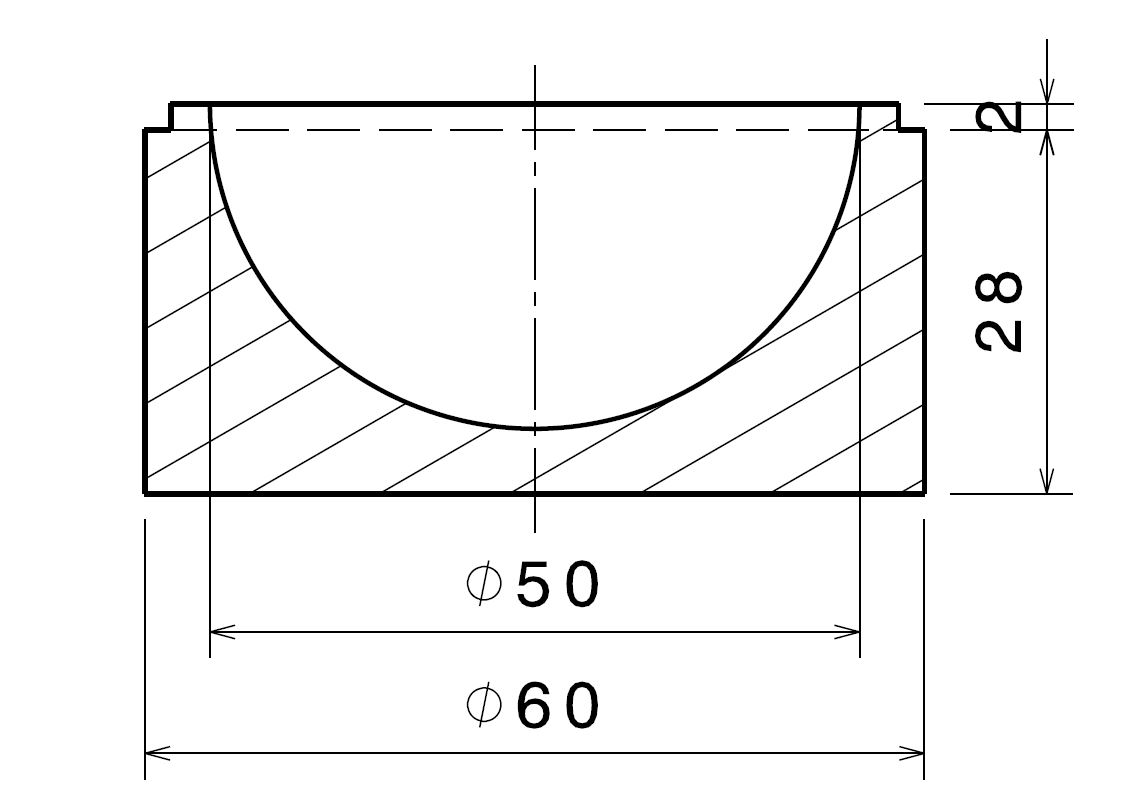
\includegraphics[width=0.48\textwidth]{figures/Chapter_1/female_mold.jpg}%
		\caption{Longitudinal section of the female mold}%
		\label{fig:female_mold}%
\end{figure}


\paragraph{Translation guide sleeve:}
It is a hollow cylinder with an inner radius $R_{in} = R_{cylinder} = 30 mm$, and a thickness of $5 mm$. where the female mold is slid in. It is slightly higher than the female mold by $5 mm$. One extremity is provided with an inner chamfer of $5°$ which ensures the concentricity between the female mold and the male mold.
\begin{figure}[H] %
	\centering%
  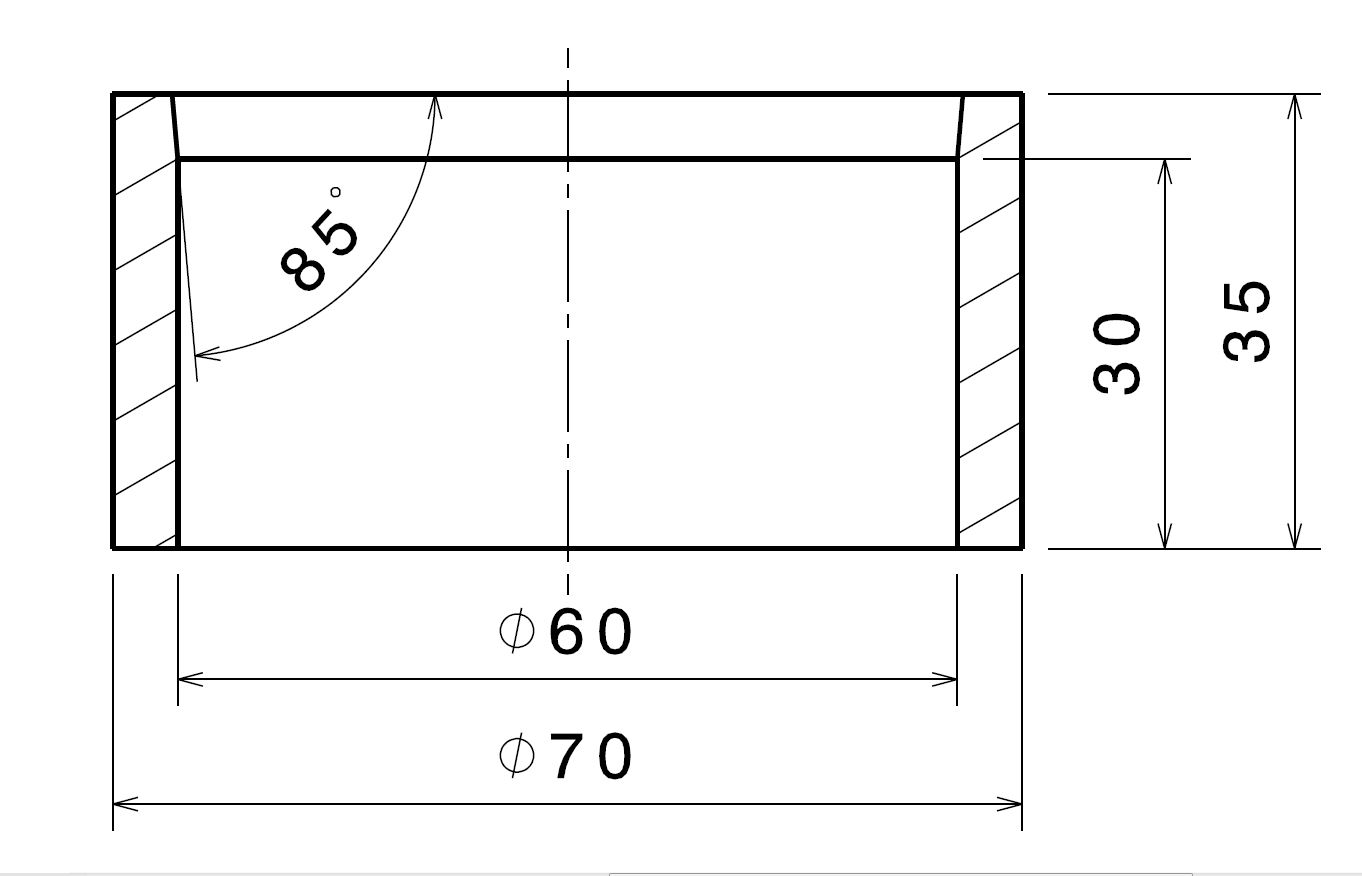
\includegraphics[width=0.48\textwidth]{figures/Chapter_1/sleeve_translation.jpg}
  \caption{longitudinal section of the sleeve}%
	\label{fig:sleeve_1}%
\end{figure}

\paragraph{Male mold:}
Figure \ref{fig:male_mold} shows the design of the male mold which consists of half a sphere of radius $R_{int}<R_{out}$, which is changed to cast different thicknesses. It is supplied with a shouldering which acts as a travel stop, its flanks have a slight angle of 5 providing a translation guide and preventing an over-center locking in combination with the guiding sleeve previously presented. The cylindrical part over the shouldering helps manipulating the mold during the casting process. Three radii have been used: $R_{int} = 18.5 mm, 20 mm, 23 mm$. 
\footnote{All the molding parts presented are made of Aluminum "`Fortal"'. The female and male molds were machined using a CNC (computerized numerical control)  machine and with a precision of $tol =\pm 0.01 mm$. The surface roughness obtained was of $R_a = 0.04$ which indicates a very good finishing.
This choice of manufacturing was unavoidable since no other alternative could produce spherical shapes with such precision conditions.}
\begin{figure}[H] %
	\centering%
  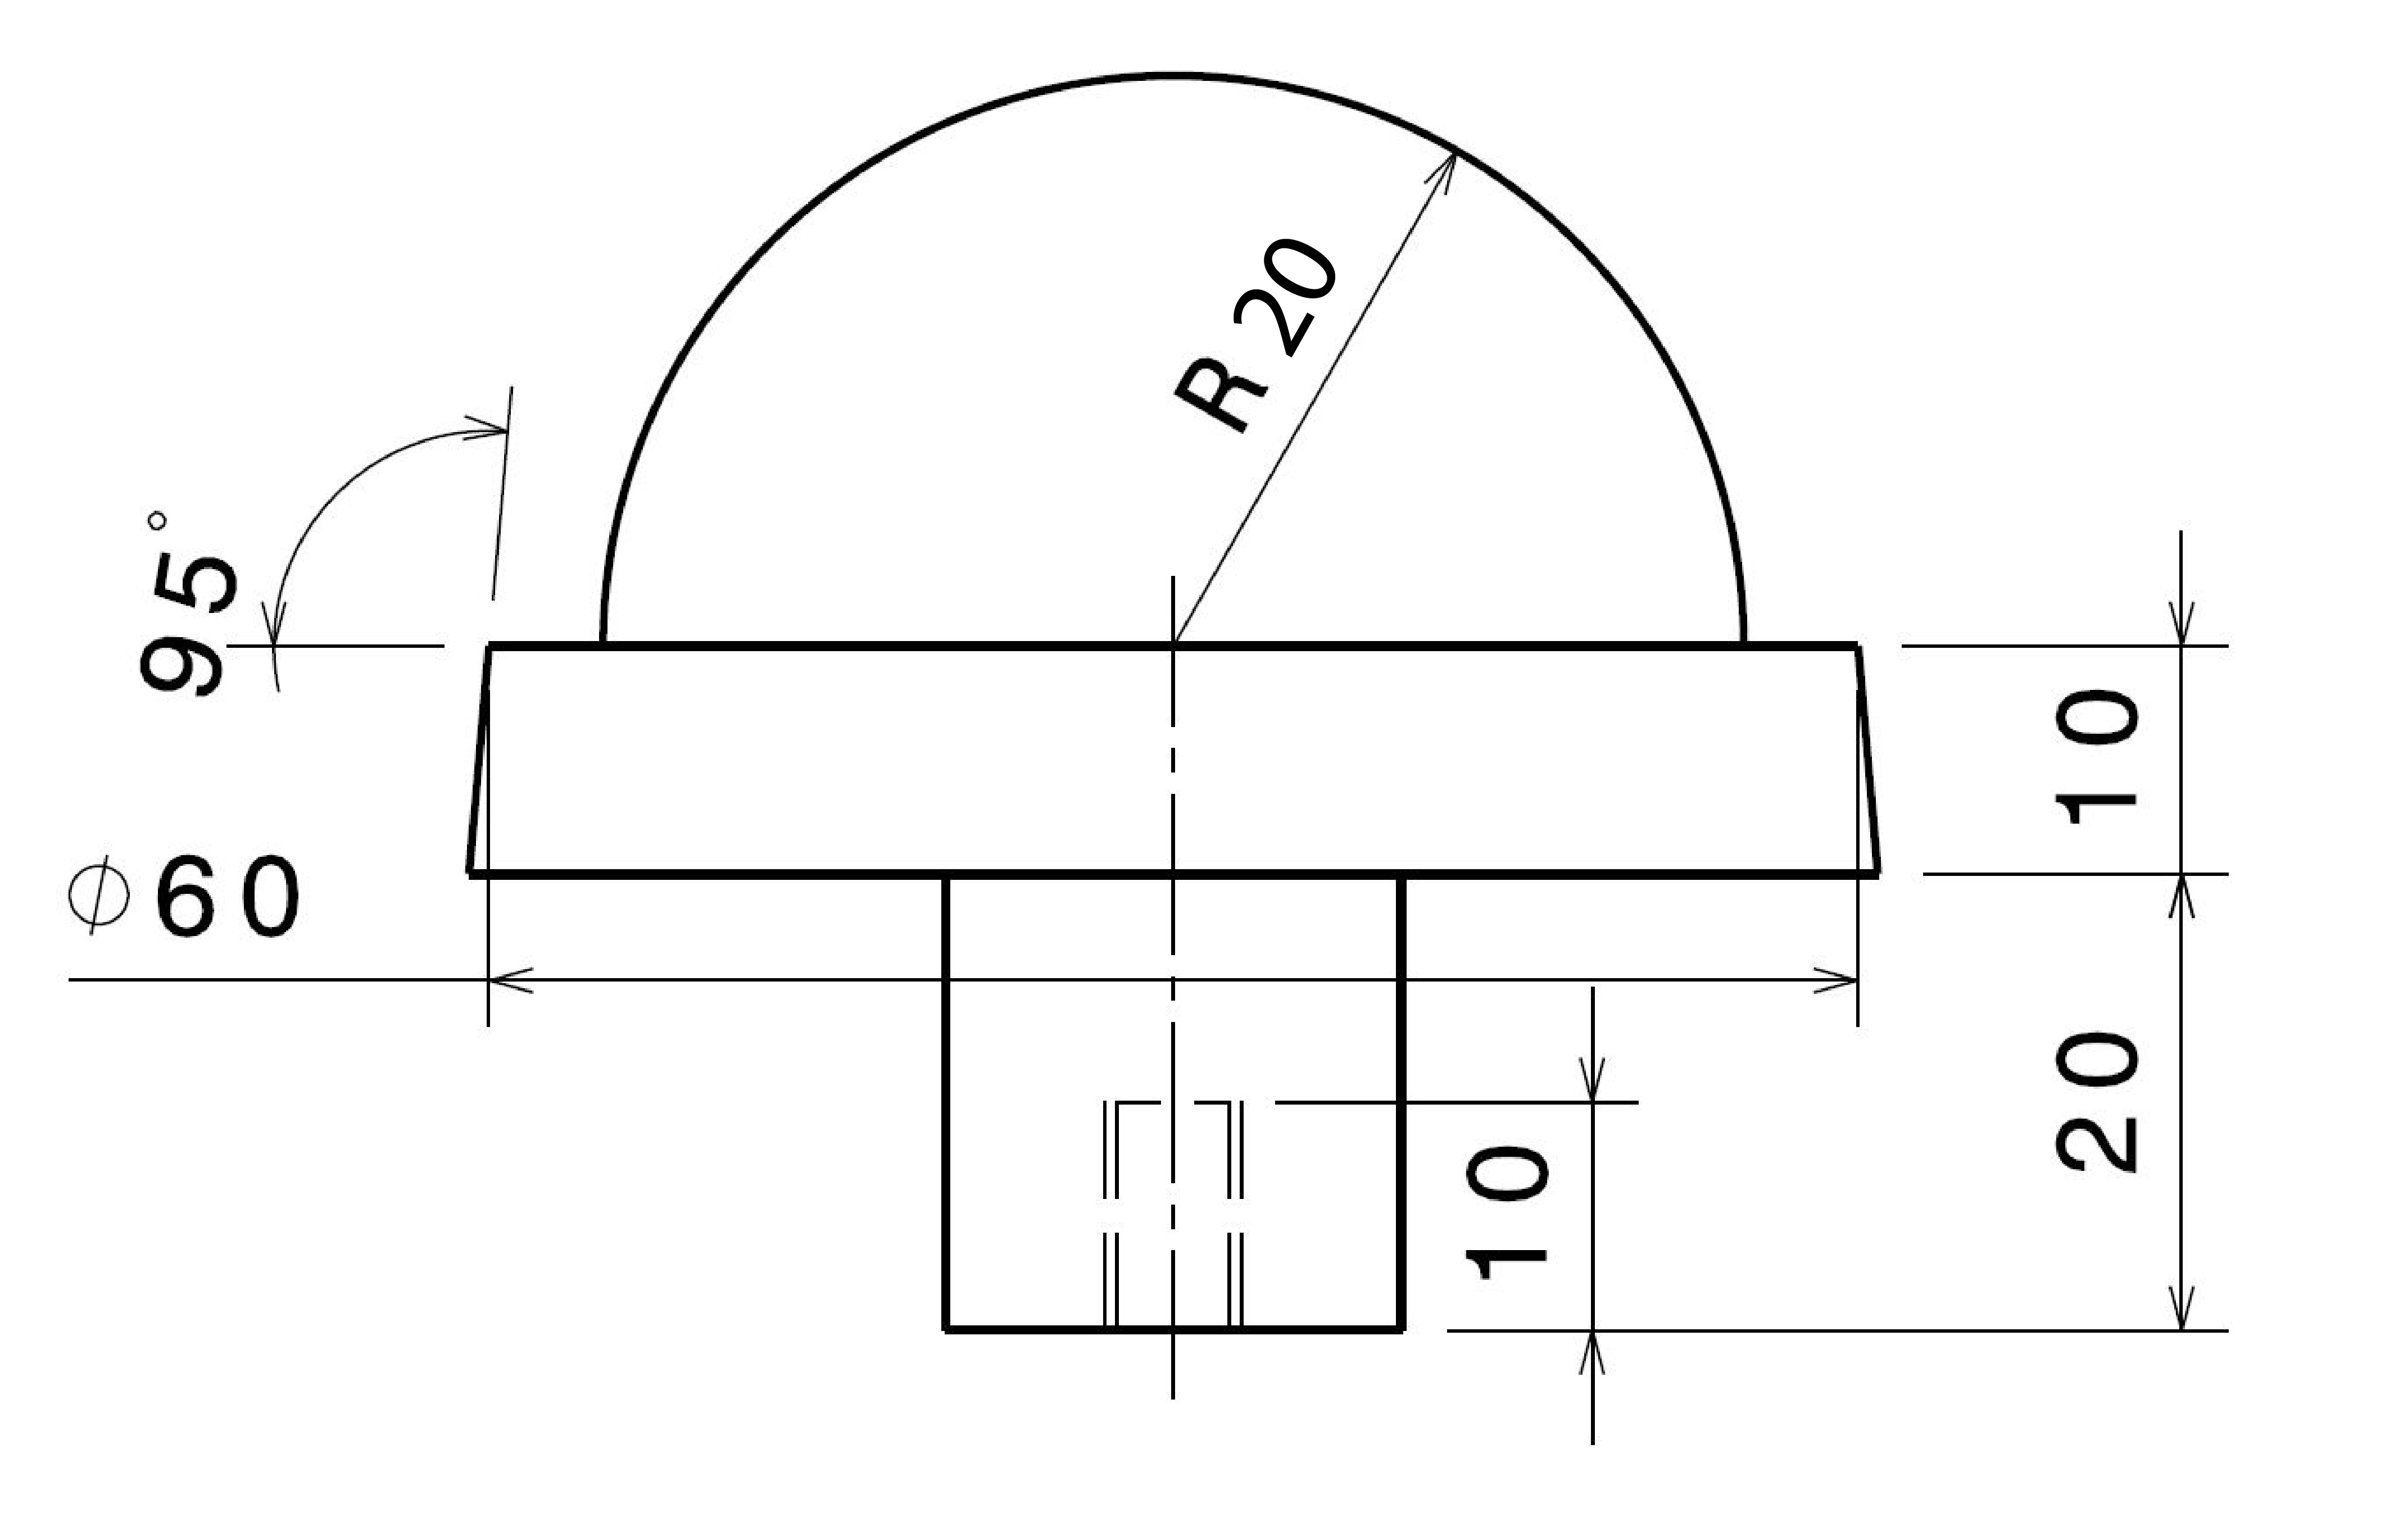
\includegraphics[width=0.48\textwidth]{figures/Chapter_1/male_mold.jpg}
	\caption{longitudinal section of the male mold}
	\label{fig:male_mold}
\end{figure}

\paragraph{Gluing sleeve:}
It is a hollow cylinder with an inner radius $R_{in} = R_{cylinder} = 30 mm$, a thickness of $5 mm$ and a height of $50 mm$. It is used during the gluing process to ensure the concentricity of the two halves of the sphere contained in the female molds which face each other.

\paragraph{Mechanical press:}
It's a simple press consisting of two metallic plates supplied with a set of threaded rods and hexagonal nuts used to apply pressure over female/male molds during the casting step to prevent bubbles from appearing during the casting step. It is also used during the gluing step on the female/female molds to ensure the contact between the two half spheres to be glued together.

\paragraph{Pasta machine:}
This machine (fig\ref{fig:pasta_maker}) consists on two rotating cylinders, with an adjustable inter-space which allows to produce layers with the desired thickness.
\begin{figure}[H] %
	\centering%
  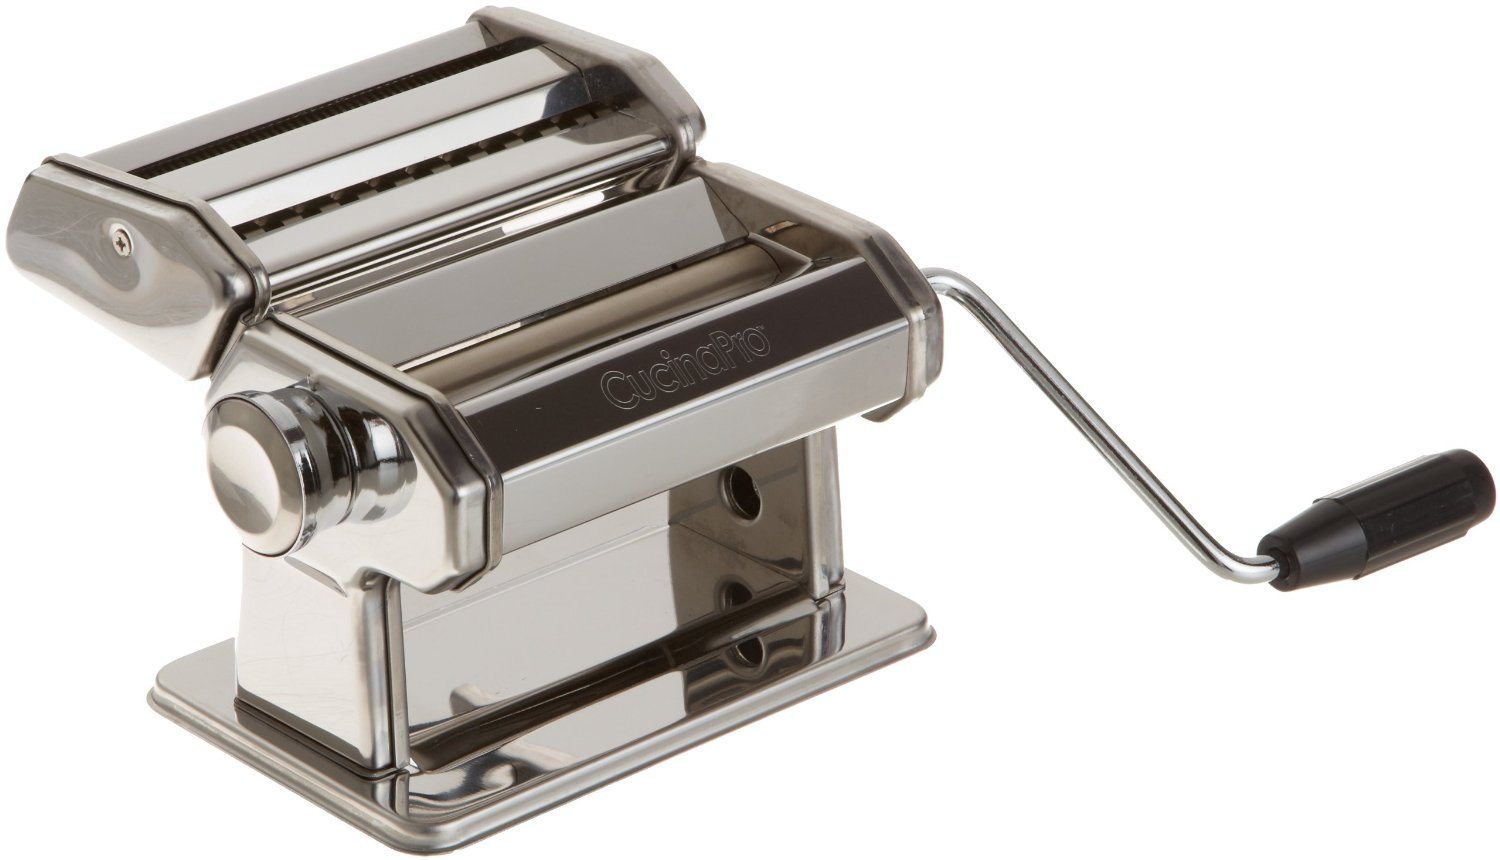
\includegraphics[width=0.48\textwidth]{figures/Chapter_1/rolling_machine.png}
	\caption{Pasta maker}
	\label{fig:pasta_maker}
\end{figure}

\newpage
\subsection{Materials and protocols}
Three materials were used in the experiments done during the study: "`Dragon Skin\textregistered 30"' which has a specific molding protocol and AJO 121 and AJO 122 which have a common molding protocol.

\subsubsection{Dragon skin\textregistered 30} 
\paragraph{}
This material is typically used to make special effects.In the case of our study, it was used to investigate the effect of the $\frac{d}{R}$ on the swimming mechanism. Its exact chemical constitution is not known, but what can be said is that it is cure liquid silicone compound, which consists of two liquid components named A and B. Component \emph{A} represents the silicon polymer chains with eventually the presence of fillers to enhance its mechanical properties. Component \emph{B} is the cross-linking agent providing bonds that link one polymer chain to another, decreasing the flexibility of the polymer chain and increasing its rigidity. Mixing these two components at room temperature, it creates a solid that takes the shape of the container it was poured in.
The typical mechanical properties of the resulting rubber are:
\begin{itemize}
	\item Shore A Hardness : 30 
	\item Specific gravity : 1.08 
	\item 100\% elastic modulus : 0.6 MPa
	\item Elongation at break : 364\%
	\item cure time (at room temperature) : 16 hours
\end{itemize}

\paragraph{Half shell casting}
\begin{enumerate}
	\item Begin by determining the mass of a shell with a outer radius of $R_{out}= 50 mm$ and a thickness $th$ which gives an internal radius $R_{int} = R_{out}-th$, The mass\footnote{In practice, this mass is increased by 50\% to take into account the eventual loss during the preparation.} of a hollow sphere is given by the following formula:
		\[Mass_{shell} = \frac{4\pi}{3}\rho_{material} (R_{out}^3-R_{int}^3) \]

	\item In a beaker, we weigh 50\% of the shell mass of component A which is the silicon polymer chain. We stir thoroughly and add 50\% of the shell mass of component B, which constitutes the cross-linking agent, we stir thoroughly.
	\item The mixture is then degassed thanks to a vacuum pump.
	\item The female and male are cleaned using acetone and 50\% of the degassed mixture is poured in the two female molds.
	\item We degas again to make sure no air was entrapped during the previous step.
	\item Each female mold is slid in the translation guide sleeve and the male mold corresponding to the desired $R_{int}$ is gently slid inside the female mold to prevent air from getting trapped.
	\item The female-male molds assembly is then pressed and locked using the press.\footnote{This step is necessary to ensure that no bubbles get trapped during the assembly.}
	\item The press is then put into an oven at 65°C to speed up the cross-linking process reducing it from 16 hours to only 20 minutes.
	
\end{enumerate}

\paragraph{Half spheres gluing:}
Once the two halves of a hollow sphere of the desired $R_{int}$ are cast. We need to glue the two halves together to obtain a complete hollow sphere of thickness $th$.
This part is critical: if the sewing is weak, it will tear apart during the buckling phase. if the sewing is thick, it means that the shape is no longer spherical. If the gluing material is not the same, we lose the homogeneity of the material and potentially create a weak zone at the sewing, which would accelerate the weakening of this zone and ultimately tear apart.
\paragraph{} 
To efficiently glue the two halves and avoid the problems stated previously. We used the same material to perform the gluing, but for that it was necessary to decrease the viscosity of the mixture and enhance its wetting properties. For this purpose, we mixed "`Pentane"' which is an organic solvent \cite{NgLee2003} with a solubility parameter similar to that of PDMS.
The following describes the protocol of gluing:
\begin{enumerate}
	\item Prepare 10g of a mixture A+B of the Dragon skin\textregistered 30 and degas it.
	\item Add 5 ml of "`Pentane"' to the mixture and stir to obtain a diluted mixture that is neither too liquid nor too viscous and pump the resulting liquid inside a syringe.
	\item Use an abrasive such as sandpaper over the gluing area of the two halves casts to make the surface rougher.
	\item Put back each cast in the female mold and align it correctly so that the gluing area is horizontal.
	\item Pour uniformly a layer of the diluted mixture using the syringe needle on the gluing area of both casts.
	\item Put one female mold inside the gluing sleeve, facing upward then slide the second one facing downward until the two gluing areas are in contact.
	\item Ensure the contact by using the mechanical press and let the cross-linking happen at room temperature for 16 hours.\footnote{This time we don't use the oven to ensure that the pressure inside the spherical hollow shell is the atmospheric pressure.}
	\item After the curing time, remove the residual thin skin circling around the sewing area.
\end{enumerate}
  

\subsubsection{AJO121/122}
\paragraph{}
The two remaining materials \emph{AJO 121} and \emph{AJO 122} were samples kindly supplied by "`\textbf{BLUESTAR silicones\textcopyright}"'.Both are hot curing silicone rubbers after addition of a vulcanization agent. The typical applications of these materials are: molding and injection molding process for technical parts (sealing gaskets,grommets), extrusion profiles (windows profiles, sleeves, tubes) and calendering operations for manufactured hoses. They were chosen to investigate the effect of solid dissipation characterized by the rebound resilience property. This pair of materials present the particularity of sharing the same elastic energy storage capacity characterized by the elastic modulus.In the case of the samples provided by "`\textbf{BLUESTAR silicones\textcopyright}"', both material present a soft white paste-like texture. The exact chemical composition of the pastes were not disclosed but what we know is that the curing agent, which is 1.25 \% of \textbf{2,4-dichlorobenzoyl peroxide}, was already mixed with the silicone polymer. The vulcanization process is temperature-controlled and is induced at 115°C.\\

The typical mechanical properties of the resulting rubbers are:
\begin{itemize}
	\item 100\% elastic modulus AJO121 / AJO122 : 2.2 MPa / 2.3 MPa
	\item Rebound resilience AJO121 / AJO122 : 45\% / 65\%
	\item Shore A AJO121 / AJO122 : 60 / 59 
	\item Specific gravity : 1.16
	\item Elongation at break AJO121 / AJO122 : 560\% / 366\%
	\item cure time (at 115°C) : 10 minutes
\end{itemize}

\paragraph{Half shell casting:}
\begin{enumerate}
	\item Begin by determining the mass of a shell with a outer radius of $R_{out}= 50 mm$ and a thickness $th$ which gives an internal radius $R_{int} = R_{out}-th$, The mass of a hollow sphere is given by the following formula:
		\[Mass_{shell} = \frac{4\pi}{3}\rho_{material} (R_{out}^3-R_{int}^3) \]

	\item Weight the calculated mass from the paste and divide it in two equal parts.
	\item Press each part at the center of the female mold.
	\item Each female mold is slid in the translation guide sleeve and the male mold corresponding to the desired $R_{int}$ is slid inside the female mold.
	\item The female-male molds assembly is then pressed and locked using the press.
	\item The press is then put into an oven at 115°C to trigger the vulcanization process, during 8 minutes \footnote{This period was reduced to 8 minutes instead of 10 minutes to avoid reaching the maximum of the cross-linking, in order to complete the gluing}.
	\item A post-curing at 200°C is needed to optimize the mechanical properties of the material, to evaporate remaining volatile substances (sub-products linked to the peroxide) and allow the sublimation of the 2,4 Dichlorobenzoic acid which manifests as a white powder at the surface of the material, at the end of the previous step.
\end{enumerate}

\paragraph{Half spheres gluing:}
The gluing using the AJO materials was very challenging for different reasons. First, the paste-like nature of the material which was not soluble in any organic solvent without compromising the vulcanization agent already mixed with the raw polymer. It also made manipulating it harder, contrary to the liquid nature of the "`Dragon Skin\textregistered 30"'. Second, we were not able to glue together two flat surfaces, due to the fact that the cross-linking process reached a maximum with the prescribed time and temperature and no biding was possible afterward.
This is the protocol followed which solved partially the problems previously stated:

\begin{enumerate}
	\item Prepare two thin layers (0.1 mm) using the "`pasta maker"' machine. Adjust their width to 10 mm and the length to $2\pi R_{out} \approx 157 mm$.
	\item Use an abrasive such as sandpaper over the gluing area of the two halves casts to make the surface rougher.
	\item Put back one cast in the female mold and align it correctly so that the gluing area is horizontal.
	\item Put uniformly a first layer on the gluing area of one cast and make sure it adhered to the surface, cut the residual width using a scalpel.
	\item Connect the remaining half (without the female mold) with the first and press to get and adhesion.
	\item Put one female mold inside the gluing sleeve, facing upward then slide the second one facing downward until the two gluing areas are in contact.
	\item Remove the female mold gently and roll the second layer around the sewing perimeter, taking care not to disconnect the two halves while doing so.
	\item Encapsulate the shell inside the two female molds and exert pressure using the mechanical press.
	\item Put the press inside the oven at 115°C for 10 minutes. Remove it and let it cool at room temperature.\footnote{The capsules produced using this protocol have an internal pressure close to $75\%$ of the atmospheric pressure.}
\end{enumerate}

\section{Spring experiment}
\subsection{Brief introduction and motives}

\paragraph{}
The purpose of this experiment is to quantify the thrust generated during the buckling and unbuckling phases when the pressure cycle is imposed externally, using a force sensor. The advantages of this method is that all the forces that are involved can be quantified using the recording images of the experiment. To do so, the capsule is attached to a spring and immersed in a tank filled with a Newtonian liquid characterized with a density $\rho$ and a viscosity $\mu$. The spring plays the role of a force sensor and prevents the spherical shell from floating to the surface due to buoyancy effects.  The buckling spot is directed in the vertical direction, to get a 1-D displacement\footnote{In theory, the buckling can happen anywhere on the capsule. In practice, the buckling happens at the same spot if the boundary conditions are not changed. This is due to the presence of a weakness in the material which decides of the buckling spot.}. Pressure cycles are applied by pressurizing the air above the liquid in which the shell is immersed. Figure \ref{fig:spring_experiment_schematic} is a representation of the spring experiment.
\begin{figure}[H] %
	\centering%
  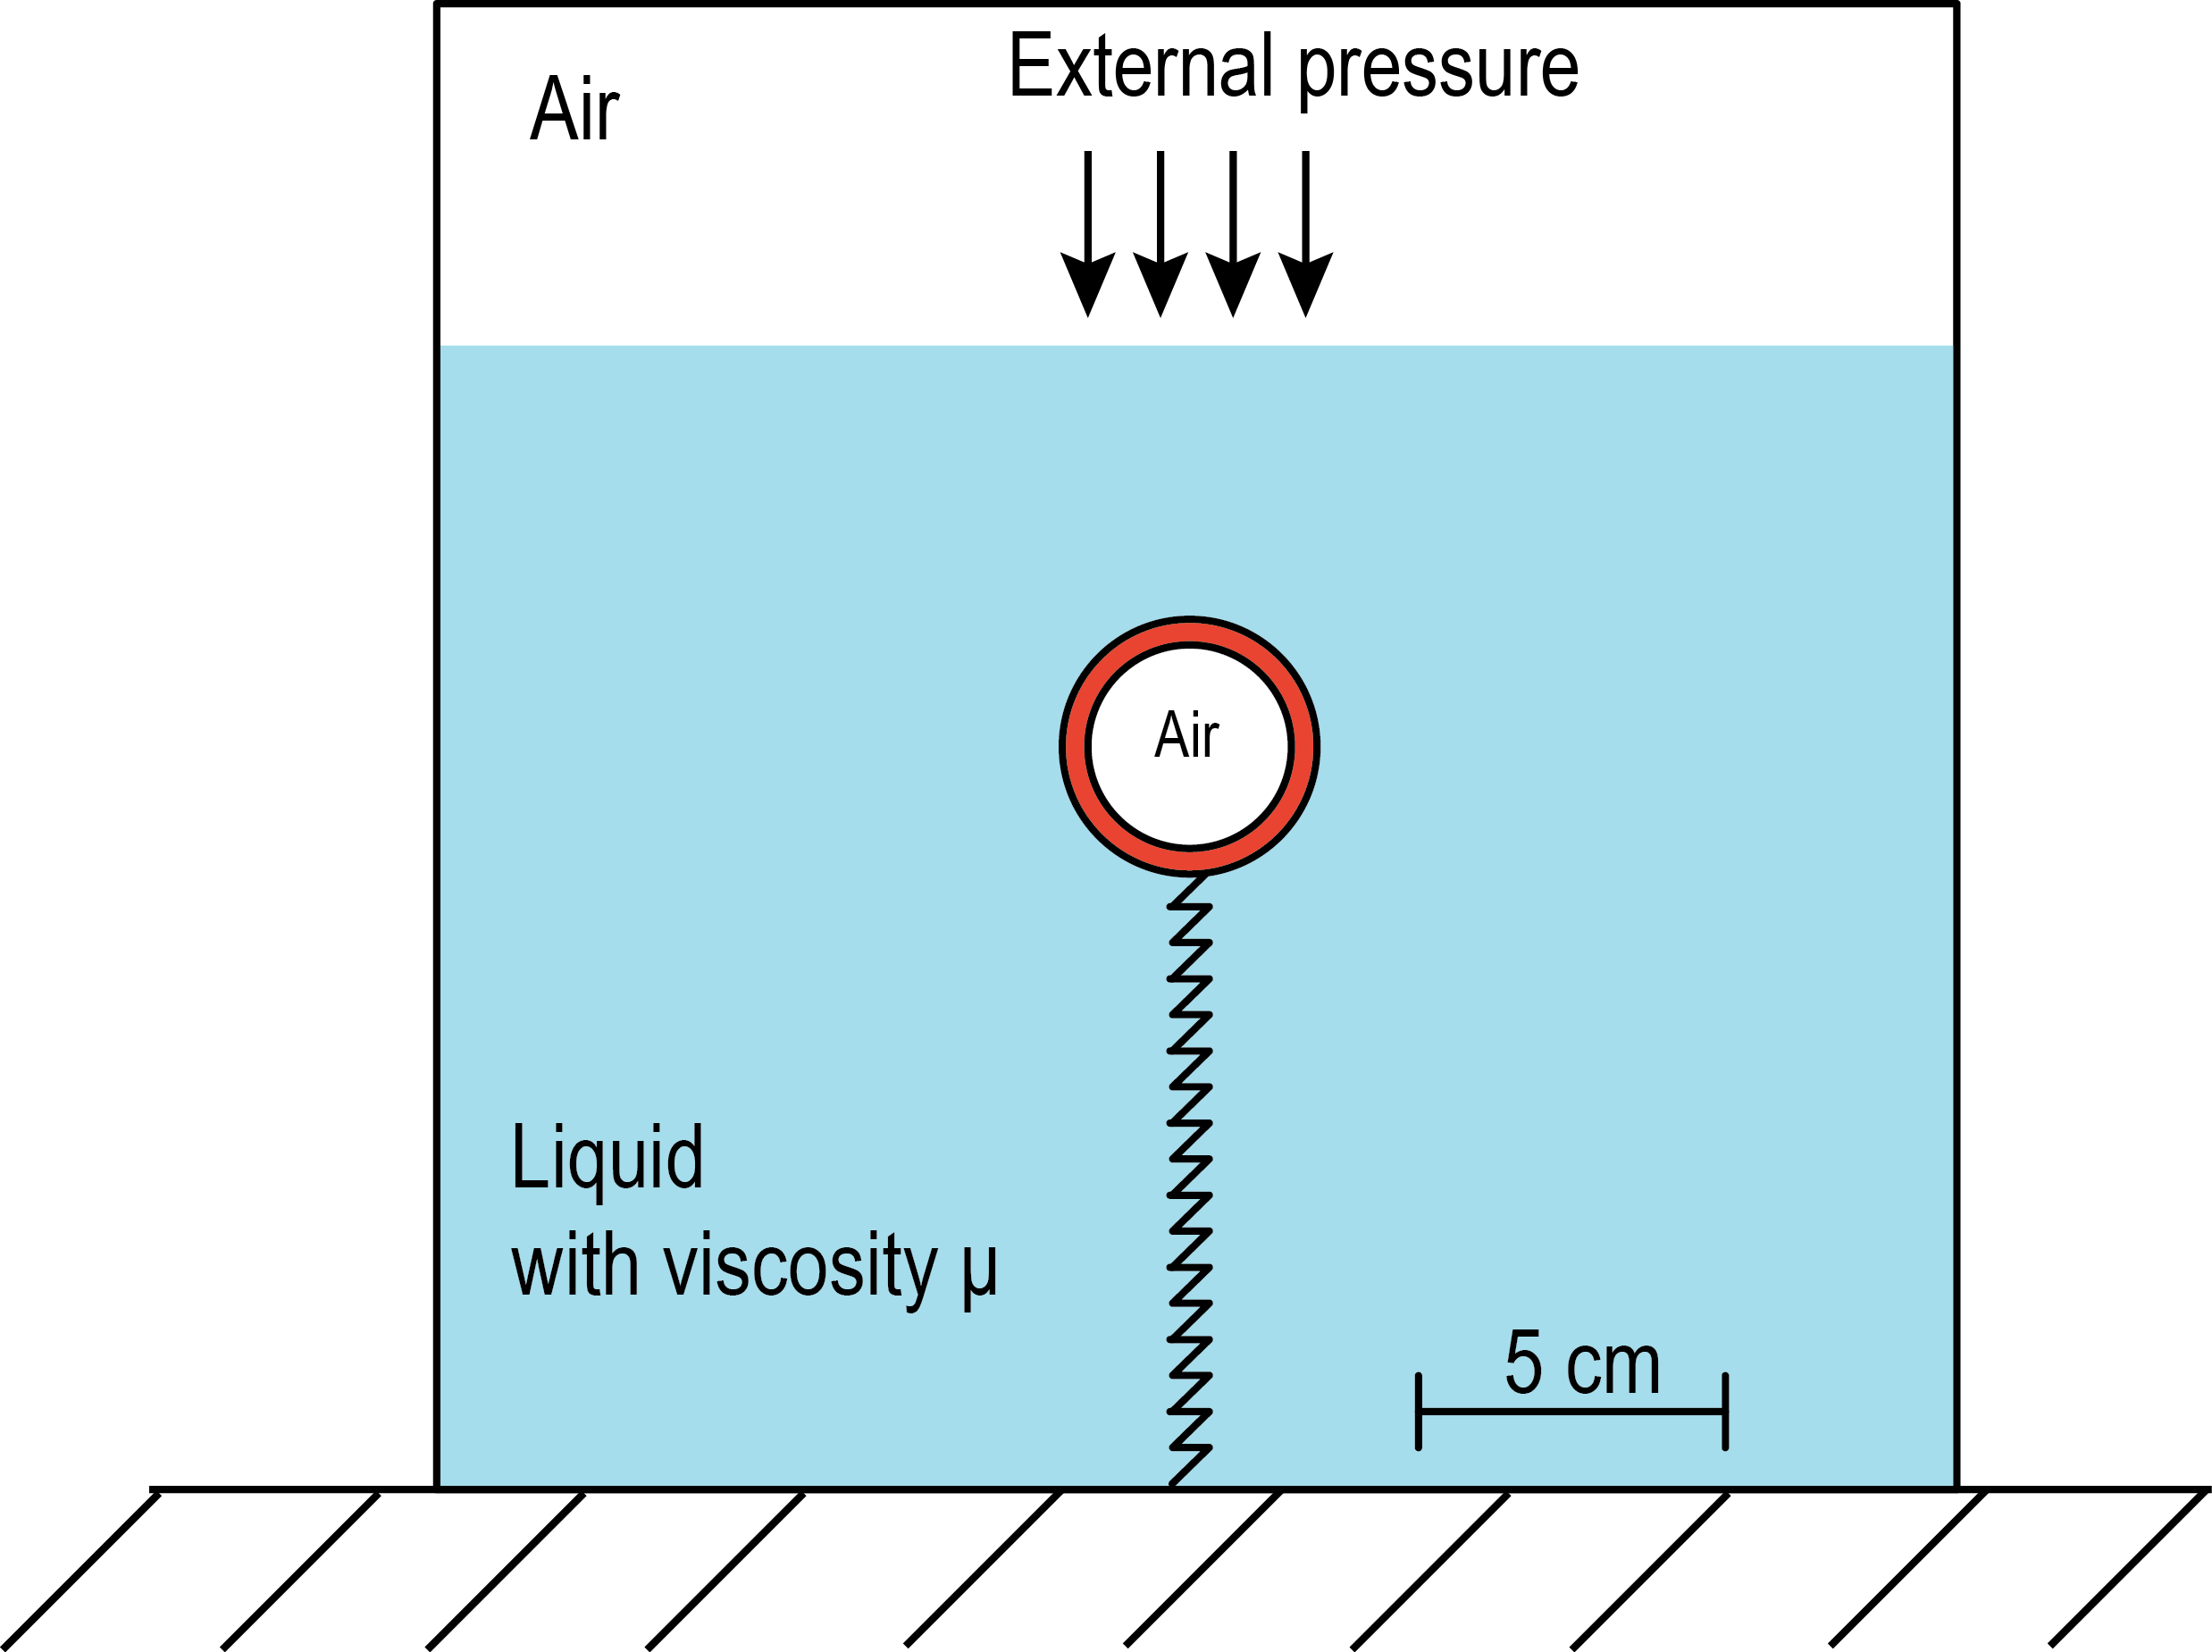
\includegraphics[width=0.73\textwidth]{figures/Chapter_1/schematic_experimental_setup.png}
	\caption{Schematics of the spring experiment}
	\label{fig:spring_experiment_schematic}
\end{figure}

\subsection{Equipment}
\subsubsection{Tank}
\paragraph{}
It consists of a cubic tank (see fig.\ref{fig:tank}) made of anodized Aluminum supplied with windows made of polycarbonate polymer. It is dimensioned to withstand an absolute pressure bigger than $3 10^5 Pa$. Its dimensions are consistent with the non-confinement conditions (CITATION) where the characteristic length of the container is close to 10 times the characteristic length of the object to be studied.
\begin{figure}[H] %
	\centering%
  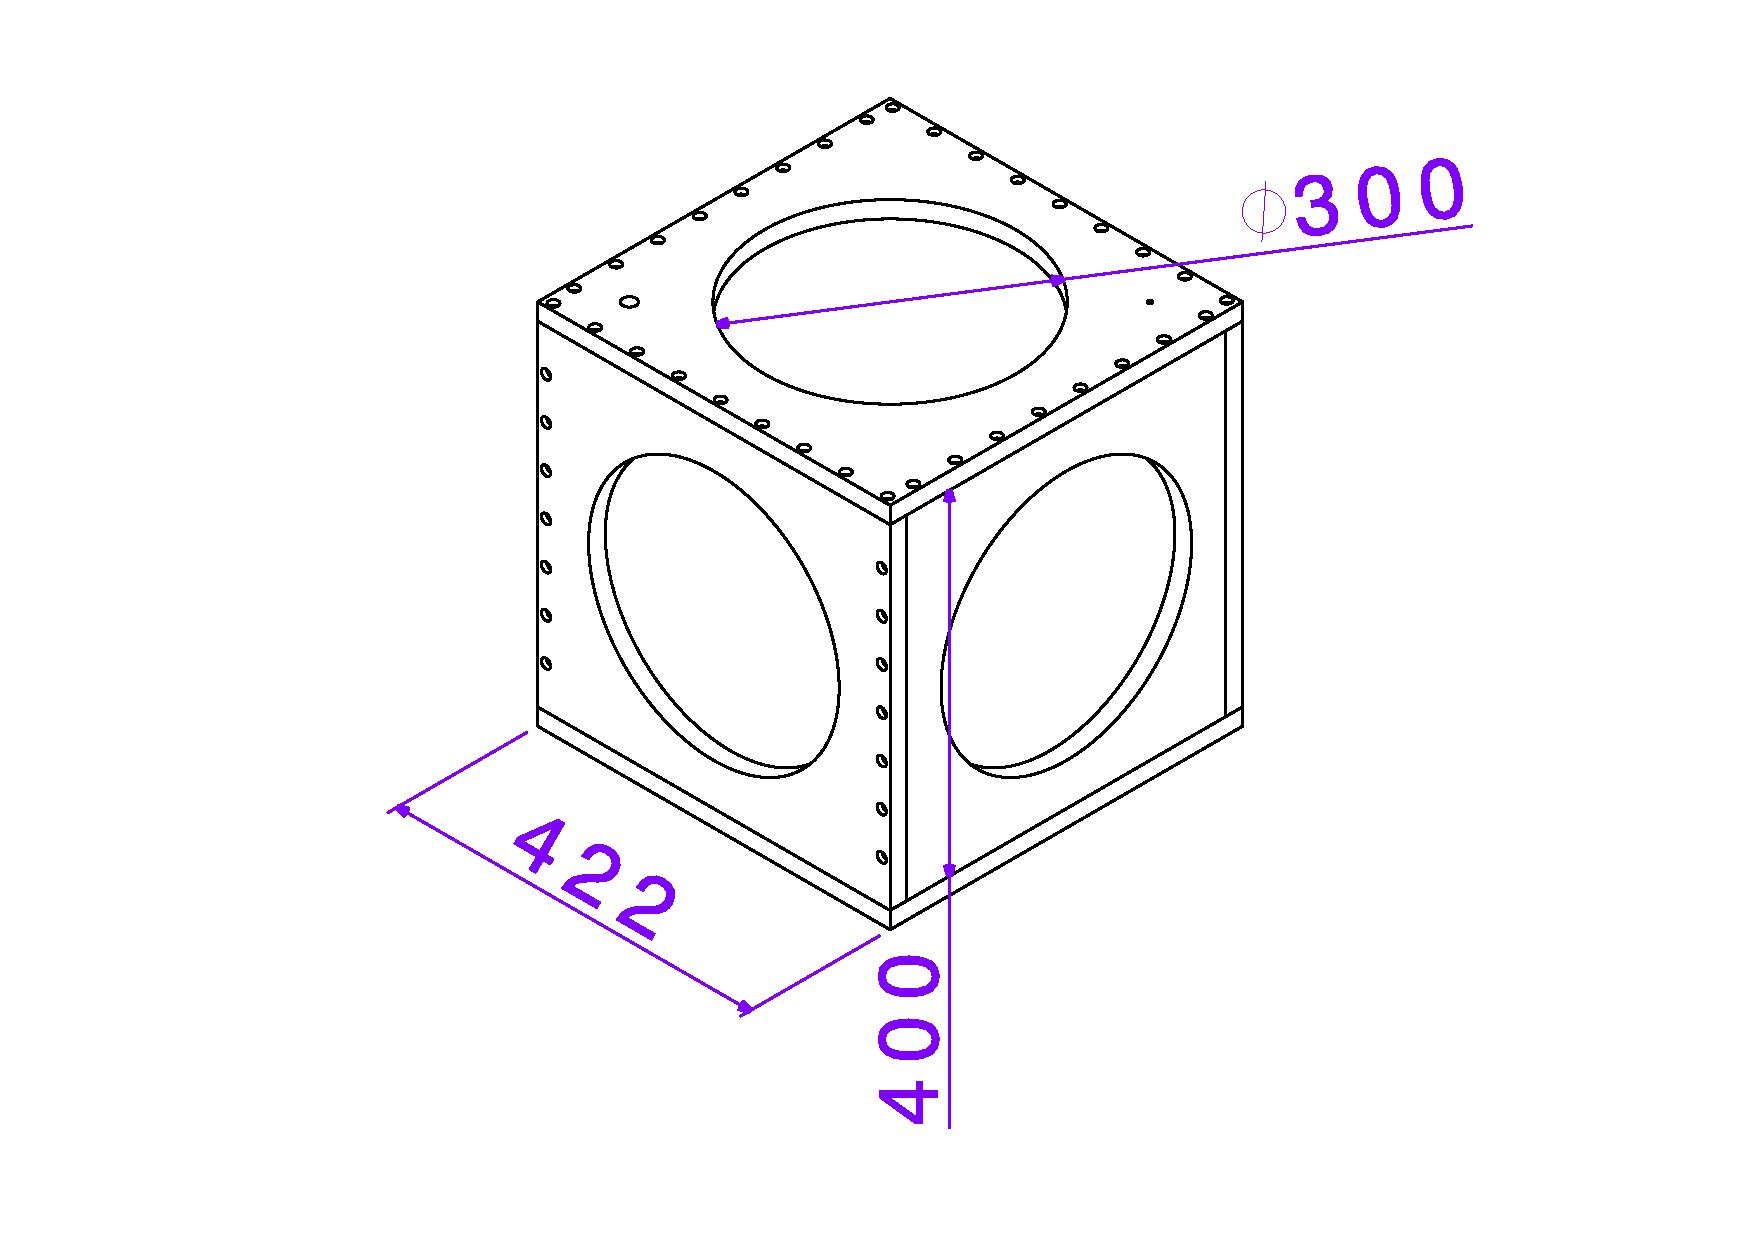
\includegraphics[width=0.73\textwidth]{figures/Chapter_1/cuve.pdf}
	\caption{Schematics of the pressurizeable tank}
	\label{fig:tank}
\end{figure}
\subsubsection{Spring}
\paragraph{}
As described earlier, the spring is used as a force sensor. The spring also allows to keep the spherical shell immersed in the liquid.
At rest, its elongation is directly proportional to the force $F_{measured} = K \Delta x$, where k is the stiffness coefficient.
\paragraph{}
In the case of our study, the spring is solicited in traction. Taking into account that the outer radius for all the capsules studied was fixed at 50 mm and that the buoyancy force is significantly larger than the weight, only one spring stiffness was needed to carry out the experiment.
The spring was dimensioned to have a total length of 200 mm at rest in water. Knowing that after the buckling, the equilibrium state reached is lower due the decrease in volume (by $\approx 20\%$, determined by preliminary results), a constraint was added to avoid the case where the spring rings would be in contact with each other which would bias the force measurement.
\paragraph{}
The characteristics provided by the manufacturer concerning the spring used in this experiment are:
\
\begin{itemize}
	\item Stiffness coefficient : 7 N/m
	\item Length at rest : 100 mm 
	\item Material : EN 10270-3 stainless steel
	\item Wire diameter : 0.5 mm
	\item External diameter: 7.93 mm
\end{itemize}

It was also provided with threaded ends to fit M6 and M4 screws. The M6 end is designed to link the spring to a fixed base at the bottom of the tank. The M4 end is designed to support a suction cup provided with a M4 screw. This suction cup is used to attach the spherical capsule to the spring.


\subsubsection{Spherical shells}
\label{sec:Spherical_shells}
\paragraph{}
The spherical shells used in this experiment are shells cast in the 'Dragon skin \textregistered 30' material. The external radius is kept constant at 5 cm and three thicknesses were explored: 2 mm, 5 mm and 6.5 mm.
The choice of these thicknesses is primarily directed by the fact that we wanted to explore the effect of stored elastic energy on the buckling mechanism and the thrust induced during the deflation and the re-inflation of the capsule. Taking into account that the stored elastic energy before the advent of the buckling instability is proportional to the ratio between the thickness and the shell radius squared \cite{cqpcritic2011} $P_c \propto (\frac{d}{R})^2$, the resulting range of variation of this geometric ratio in this experiment, ranges from $6.4 10^{-3}$ to $6.76 10^{-2}$.
A lower value of this parameter was tried (taking a thickness of 1 mm) but it resulted in a spontaneous buckling when immersed, due to the static pressure.
A higher value of of this parameter was tried (taking a thickness of 7.5 mm) but it was not possible to reach the pressure high enough to produce a buckling in the range of the operable pressure [0, 2] bars.
\paragraph{}
Special measure were taken to conduct experiments on the 2mm thick shell, due to the fact that once attached to the suction cup that ensures the link with the spring, the shell gets deformed at the attaching point by buoyancy effects which lower locally the curvature radius, creating a weak spot \cite{cqpcritic2011}. An imperfection was introduced at the casting, by reducing locally the thickness of the shell. Practically, the shell thickness was reduced of 0.1 mm over a circular surface with a 10 mm diameter.
\paragraph{}
One of the properties of the material used is its semi-transparency when light is shone on it. which is an important feature to determine the volume of the concave shapes resulting after the buckling.

\subsubsection{Pressure controller}
\paragraph{}
Since deflation and re-inflation cycles of the shell are actuated by applying a difference of pressure between the inside and outside, it was necessary to use a pressure controller.
\paragraph{}
A pressure controller is not an air compressor, it needs a high pressure input. The user sets the pressure wanted using a piece of software which in turn, communicates with the hardware assigning the desired command. The pressure controller then, opens its valves and regulates the in/out air flux until the desired pressure is reached, using a pressure sensor which measures a relative pressure to the reference: the room atmospheric pressure.
\paragraph{}
The equipment used during this experiment is the OB1 flow control system manufactured by Elveflow\textcopyright. This system is supplied with four channels (fig.\ref{fig:ob1}), three channels operate between 0 and 2bars (relative pressure) and one channel operates between -1 and 1 bar and requires a vacuum pump to reach -1 bar.
In the spring experiment, the external pressure is the control parameter, therefor only a 0-2 bar channel was used.
As stated earlier, a pressure source is necessary to be able to use the "`OB1"' pressure controller, and in this case a 6 bar pressure source is used.
\paragraph{}
The pressure is controlled thanks to a very user-friendly interface, which allows to apply different kind of pressure signals such as: constant, ramp, sinusoidal, square signals. It also allows programing sequences using the previously stated signals, but also wait time, triggers and loops. This particular function was helpful to implement reproducible pressure cycles during the spring experiment.
\paragraph{}
To ensure the proper functioning of the pressure controller, two air filters were used: one upstream, to filter the air between the pressured air supply and the "`OB1"' and one downstream to filter the air between the "`OB1"' and the tank, where liquid vapor can affect the equipments of the "`OB1"' during the pressure regulation phase.
The air filters used consist in a 5$\mu$m pore size pneumatic filter which removes liquid and solid contaminants. It is supplied with drain that can be opened as needed to drain condensed contaminants.
\begin{figure}[H] %
	\centering%
  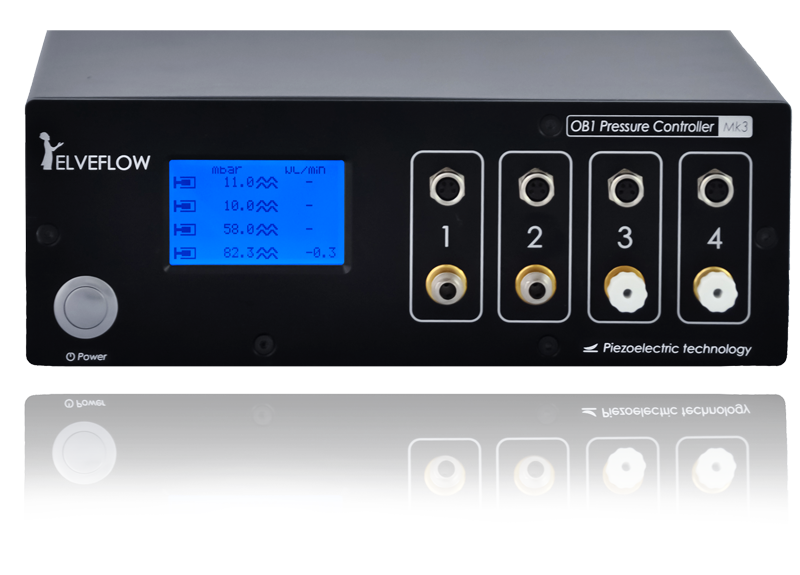
\includegraphics[width=0.48\textwidth]{figures/Chapter_1/OB1.png}
	\caption{OB1 pressure controller}
	\label{fig:ob1}
\end{figure}
\paragraph{Notes}
This pressure controller is not supposed to be used in such conditions, operating on rather large air volumes. One of its inconveniences was its time response with a max air-flux dimensioned for micro-fluidic experiments. We bought a pressure controller intended to work with large volumes but it was not supplied with neither any power supply nor any software and necessary electronics to control it with a computer. The fact that we were not investigating the actuation frequency role in the physics and the impossibility to control negative relative pressures, comforted us into using the plug and play solution "`OB1"'.

\subsubsection{Camera,lenses and light sources}
\paragraph{Camera:}
Taking into account the fast nature of the instability, where the shells undertakes a deformation of almost a radius, in less than 5 ms, it was necessary to use a high-speed camera.
The camera used for this purpose is the Phantom\textcopyright Miro 310, its main characteristics are the following:
\begin{itemize}
	\item Resolution: One megapixel, 1280x800.
	\item Full resolution speed: 3260 frame per second (FPS).
	\item Sensor: CMOS sensor with 20 $\mu$m pixel size, 12-bit depth gray-scale colors.
	\item Memory: 6GB, with 2.3 seconds record time at maximum frame rate.
	\item Communication: Gb Ethernet for control and data.
\end{itemize}
\paragraph{}
It is supplied with a software which allows the control of these parameters and also triggering and storing images.
\paragraph{Lenses:}
A lens with high iris opening value is necessary to capture images at high speed with low light exposure. It was necessary to capture a large field which contains an object of 50 mm plus part of a spring which moves during the process. This is why a fixed focal length $f= 50$ mm with a maximum aperture of f/1.4 was selected, from the lens manufacturer Zeiss\textcopyright.

\paragraph{Light source:}
Three parameters were to take into account for the choice of light sources:
\begin{enumerate}
	\item A stable source of light with no variation of light intensity was required to be able to use the 2D image registration algorithm "`UnwrapJ"' to correct the deformation of the tank windows due to pressure.
	\item A powerful intensity is required to be able to record at high speed.
	\item A homogenous light source is needed to be able to correctly extract the edges of the shell from the images.	
\end{enumerate}
To do so, two 30x30 daylight balanced led-based panels were used providing 6560 lumen, disposed as shown in figure \ref{fig:schematics_spring}. The one at the back is tuned at full power to highlight the complete ball-spring system and a filter is added to diffuse light and avoid seeing the individual leds. The one upfront is used with 25\% of its power, in order to see the concavity, once the shell is buckled.
\begin{figure}[H] %
	\centering%
  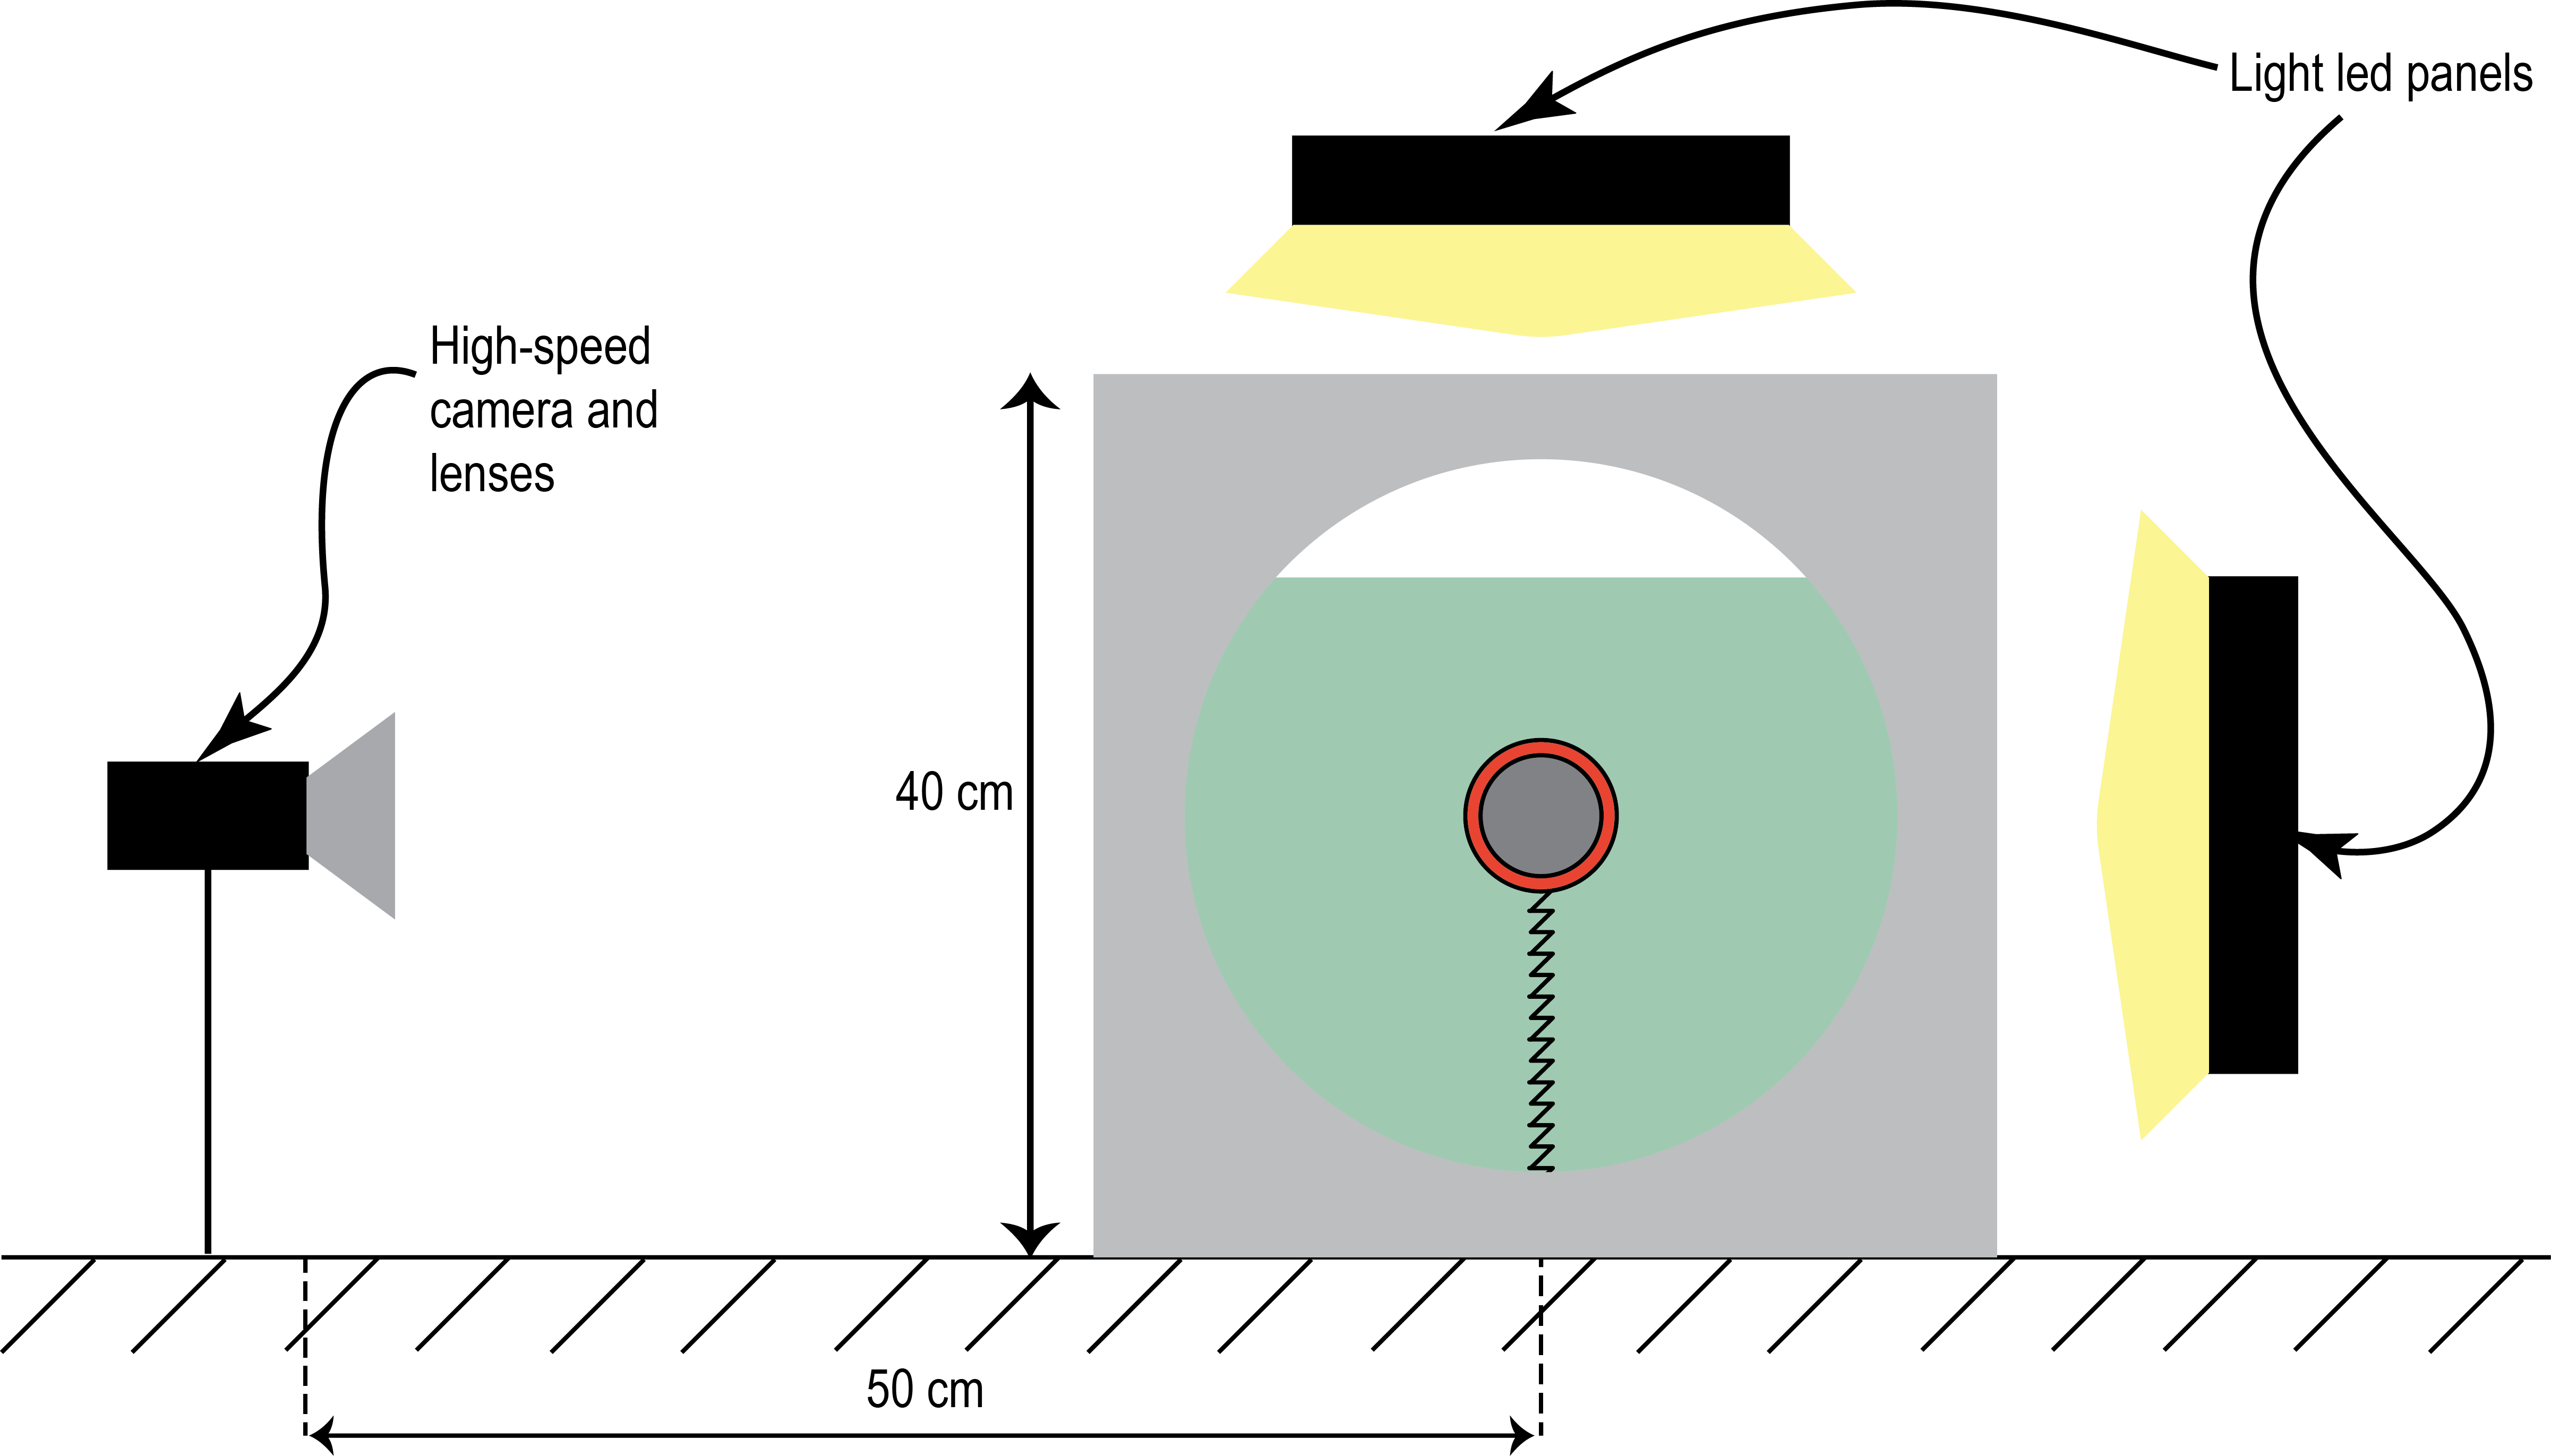
\includegraphics[width=0.73\textwidth]{figures/Chapter_1/schematic_experimental_setup_light_lenses.png}
	\caption{Representation of the light and camera dispositon}
	\label{fig:schematics_spring}
\end{figure}
\newpage
\subsection{Experimental process}
\subsubsection{1-D orientation}
\paragraph{}
Theoretically, the buckling instability nucleates randomly  on the surface of the shell. Practically, this instability always occurs at a specific spot of the elastic shell which represent its weak spot, when the boundary conditions are not changed \footnote{Experimentally, when the shell is in contact of a wall, the buckling spot occurs at the contact point, due to some change in the shell stress.}.
\paragraph{}
To properly conduct a force measurement, using a spring, it is necessary to align the buckling spot in the spring axis to obtain a 1-D displacement. To do so, a series of preliminary experiments are conducted to determine precisely the buckling spot:
First, mark the shell surface with 12 distinctive symbols, then put the marked ball inside the tank and apply a pressure to induce the buckling instability. Once buckled, define the closest symbol to the concavity center resulting from the buckling. Link the shell to the suction cup fixed on the spring, in a way to have the buckling spot aligned to the spring and mark the position of the guessed buckling spot and the attaching area and pressurize the the tank to trigger the buckling again. Measure the angle between the spring axis and the concavity and repeat the operation until a 90° angle is achieved. 
\paragraph{}
This step also allows to determine the critical pressure at which the buckling and unbuckling occur.
\subsubsection{Experimental protocol}
\paragraph{}
We used three fluids in this experiment, and in each fluid, three capsules were investigated \ref{sec:Spherical_shells}.
The main characteristics of the fluids used are shown in table \ref{tab:fluid_carac_spring}. The following experimental protocol is applied for each fluid.
\begin{table}[H]
	\centering
		\begin{tabular}{|l|c|r|}
			\hline
			Fluid & Density (Kg.m$^{-3}$) & Viscosity (Pa.s)\\
			\hline
			Glycerol & 1250 & 1.37 \\
			\hline
			Water & 1000 & 10$^{-3} $\\
			\hline
			Air &  1.2 & 10$^{-6}$\\
			\hline
		\end{tabular}
	
	\caption{Fluids used in the experiments and their main properties at room temperature.}
	\label{tab:fluid_carac_spring}
\end{table}
\paragraph{Quasi-static experiments:}
We noticed, during the first experiments done with the spring that the shape of a shell submitted to a constant pressure P, continues to slightly evolve in time due to the relaxation of the material through creep. To investigate this effect, quasi-static experiments were conducted by submitting the shell to a pressure cycle which evolves at a slow rate. Practically, a step-like cycle was applied knowing the buckling and unbuckling critical pressures.\\
Figure \ref{fig:quasi_static_pressure_cycle} shows a qualitative example of such step-like cycle where the step width represents the amount of time waited at each pressure step\footnote{by varying this step width, we can evaluate its importance and how it impacts the instability dynamics}.
First, an image is recorded at (P=0), then the pressure is increased by a pressure step and is kept constant during a time $T=step width$, at the end of this time an image is recorded. This process is repeated until nearing the pressure at which the buckling occurs which can slightly vary from an experiment to another, the pressure is then gradually increased by smaller steps\footnote{The smaller steps are necessary in order to keep the pressure constant at the buckling and unbuckling phases, to independently study the buckling and unbuckling dynamics.}
 and when arriving to a critical pressure where the buckling occurs, the camera is triggered and a movie is recorded at 5000 FPS \footnote{Figure \ref{fig:quasi_static_pressure_cycle} shows a longer time at the buckling and unbuckling phases to count for the time necessary to save the resulting movies, which takes about 8 minutes}. An image is taken at the end of the buckling phase, in order to record the state to which the capsule has relaxed to, following the buckling.
The pressure is decreased following the same procedure until nearing the critical pressure at which the unbuckling occurs and the same procedure is followed for the buckling phase. After that, the pressure is decreased until reaching zero.
This protocol is performed for each step width, and there are 2 of them: 10 minutes and 1 minute. 10 minutes, represents the time after which the final state of relaxation is reached and any change that might occur cannot be perceived within our experimental precision. This limit is specific to the material used. The 1 minute time was added to measure the rate at which this relaxation happens.\\
   
\begin{figure}[H] %
	\centering%
  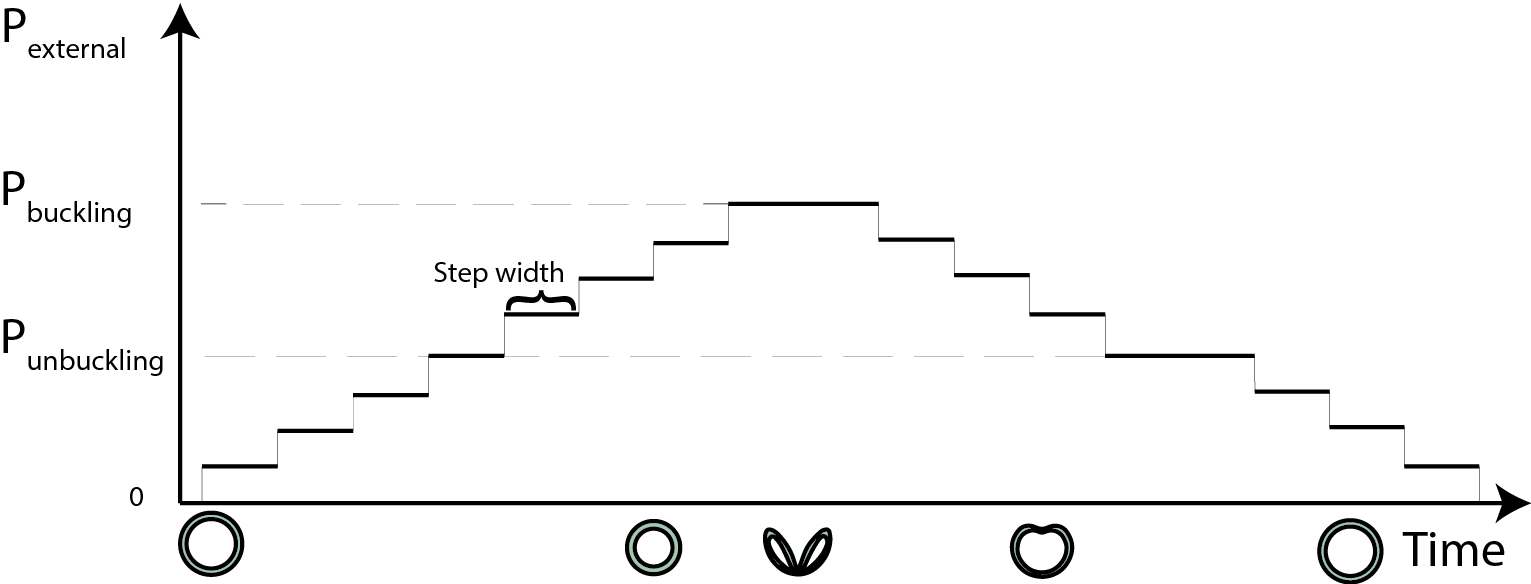
\includegraphics[width=\textwidth]{figures/Chapter_1/quasi_static_pressure_cycle.png}
	\caption{Qualitative representation of pressure cycles applied for the quasi-static experiments}
	\label{fig:quasi_static_pressure_cycle}
\end{figure}
\paragraph{Dynamic experiments:}
In the second set of experiments, step width is shortened to 20 seconds\footnote{Time necessary to save images to the computer}, and a similar cycle is applied with the exception of the phase between buckling phase and the unbuckling phase where the depressurization rate was varied, to investigate the production of thrust during the rolling. 
Figure \ref{fig:quasi_static_pressure_cycle} shows a qualitative example of a pressure cycle applied for the dynamic set of experiments. The parameter $\alpha$ corresponds to the depressurization rate to get from the buckling pressure to near the unbuckling pressure. Three different rates are applied.
\begin{figure}[H] %
	\centering%
  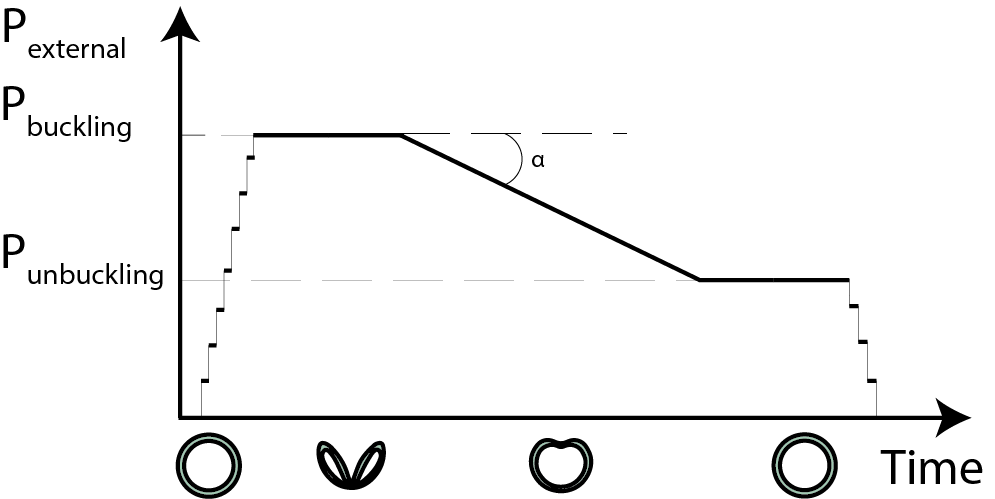
\includegraphics[width=\textwidth]{figures/Chapter_1/dynamic_pressure_cycle.png}
	\caption{Qualitative representation of pressure cycles applied for the dynamic experiments}
	\label{fig:dynamic_pressure_cycle}
\end{figure}
The fluid temperature is measured at the beginning of the pressure cycle and at its end. These temperature measurements are then, used to properly characterize the viscosity of the medium, by taking a sample and perform rheological measurements, thanks to a rheometer.\\
The tables \ref{tab:Experimental_pressure_cycle_parameters_in_glycerol},\ref{tab:Experimental_pressure_cycle_parameters_in_water} and \ref{tab:Experimental_pressure_cycle_parameters_in_air} summarize the control parameters of the pressure cycle for each $\frac{d}{R}$, in each fluid.
\begin{table}[H]
	\centering
		\begin{adjustbox}{width=\textwidth}
			\begin{tabular}{|c|c|c|c|c|}
				\hline
				Capsules & Buckling pressure (mbar) & Unbuckling pressure (mbar) & Depressurization rates (mbar.s$^{-1}$) & Temperature (Celsius) \\
				\hline
				$\frac{d}{R} = $ & 100 & [70,80] & -1, -10, -20 & [20,21.5]\\
				\hline
				$\frac{d}{R} = $ & [780,790] & [380,390] & -1, -10, -15 & [24.5,26]\\
				\hline
				$\frac{d}{R} = $ & [1350,1450] & [620,660] & 100 mbar steps, -1, -10 & [25,26]\\
				\hline
			\end{tabular}
		\end{adjustbox}
	
	\caption{Experimental pressure cycle parameters in glycerol}
	\label{tab:Experimental_pressure_cycle_parameters_in_glycerol}
\end{table}

\begin{table}[H]
	\centering
		\begin{adjustbox}{width=\textwidth}
			\begin{tabular}{|c|c|c|c|c|}
				\hline
				Capsules & Buckling pressure (mbar) & Unbuckling pressure (mbar) & Depressurization rates (mbar.s$^{-1}$) & Temperature (Celsius) \\
				\hline
				$\frac{d}{R} = $ & [100,110]& [75,85] & -1, -10, -20 & [23,23.5]\\
				\hline
				$\frac{d}{R} = $ & 780 & [360,370] & -1, -10, -20 & [20,23.2]\\
				\hline
				$\frac{d}{R} = $ &  \multicolumn{4}{c|}{Experiments were not possible due to the non visibility of the buckling concavity in water.}\\
				\hline
			\end{tabular}
		\end{adjustbox}
	
	\caption{Experimental pressure cycle parameters in water}
	\label{tab:Experimental_pressure_cycle_parameters_in_water}
\end{table}

\begin{table}[H]
	\centering
		\begin{adjustbox}{width=\textwidth}
			\begin{tabular}{|c|c|c|c|c|}
				\hline
				Capsules & Buckling pressure (mbar) & Unbuckling pressure (mbar) & Depressurization rates (mbar.s$^{-1}$) & Temperature (Celsius) \\
				\hline
				$\frac{d}{R} = $ & [100,110]& [70,80] & -1, -1, -2 & [23.5,25]\\
				\hline
				$\frac{d}{R} = $ & [850,900] & [380,480] & -1,-2,-2.5 & [24.5,26]\\
				\hline
				$\frac{d}{R} = $ & 1570 & 790 & -1 & 23 \\
				\hline
			\end{tabular}
		\end{adjustbox}
	\caption{Experimental pressure cycle parameters in air}
	\label{tab:Experimental_pressure_cycle_parameters_in_air}
\end{table}


\paragraph{Distortion correction:}
When static pressure is applied inside the tank used for the experiment, its windows made out of polycarbonate bend. This bending creates a sort of a barrel distortion which depends on the pressure applied inside the tank (fig.\ref{fig:barrel_distortion}). This distortion alters the images recorded during the experiment and ultimately any distance measurements extracted from them.
\begin{figure}[H] %
	\centering%
  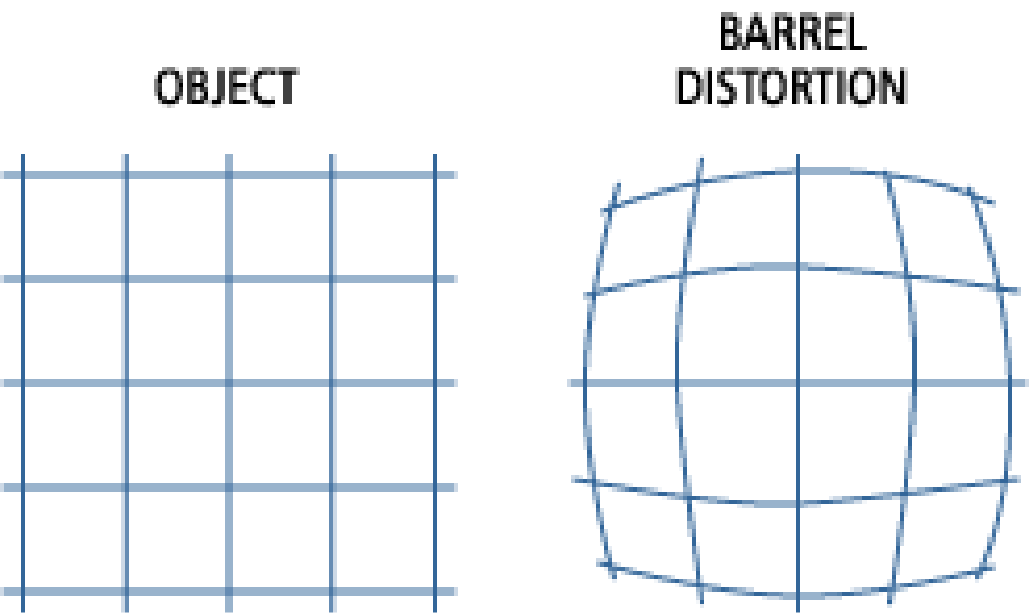
\includegraphics[width=0.48\textwidth]{figures/Chapter_1/barrel_effect.png}
	\caption{Qualitative representation of a barrel distortion}
	\label{fig:barrel_distortion}
\end{figure}
 Two possibilities to correct this effect were considered: either modeling the bent window as a lens and characterize it as function of the pressure, or applying a numerical method to find the deformation of the image between the rest state where the relative pressure is zero and a state at pressure P. Once found, this deformation matrix is inverted and we can transform a distorted image to a non-distorted one. The latter solution was adopted, because it is less time-consuming knowing an algorithm has already been implemented in ImageJ registration plugin called "`bUnwrajJ"'.
To calibrate the correction, a damier was placed at the same position as the spring-ball system, and images were recorded for each pressure step, used during experiments in one fluid\footnote{This operation is renewed each time we fill the tank with a new fluid, because the camera-tank position may change during the emptying phase}.




\subsection{Image treatment}
\paragraph{}
 The image treatment is the basis of the measurement conducted in the spring experiment, since every every physical quantity of interest is extracted from the images. But before extracting these quantities from the images, a correction of the windows distortion due to the pressurization of the tank was necessary.
\subsubsection{Image calibration due to window distortion}
\paragraph{}
As mentioned earlier, we faced a problem when pressure was applied inside the tank, inducing an error on the distances measured directly from the distorted images which depends on the camera positon in regard to the window, the spring-ball position in regard to the window and the pressure inside the tank.For example, an estimation of this deformation between at (P = 1000 mbar), by measuring a horizontal central line between the image at (P=0) and at (P=1000 mbar) yields an elongation of:
\begin{align}
	\epsilon_{horizontal} = \frac{\Delta L}{L_0} = 2\%
\end{align}
\paragraph{Calibration step} 
To correct it, we calibrated this distortion by taking an image of a damier inside the tank at each pressure step. 
 From each image, we extracted a deformation matrix that links the rest state at (P=0) to the image at (P=p$_{image}$) and the deformation matrix is inverted to get the transformation needed to transform the image at (P=p$_{image}$) into the image at (P=0), using an algorithm implement in the registration plugin category of ImageJ, called "`bUnwrapJ"'.
\paragraph{}
"`bUnwarpJ"' is an algorithm for elastic and consistent image registration developed as an ImageJ plugin. It performs a simultaneous registration of two images, A and B. Image A is elastically deformed in order to look as similar as possible to image B, and, at the same time, the "inverse" transformation (from B to A) is also calculated so a pseudo-invertibility of the final deformation could be guaranteed (fig\ref{fig:scheme_bunwrapJ}).

\begin{figure}[H] %
	\centering%
  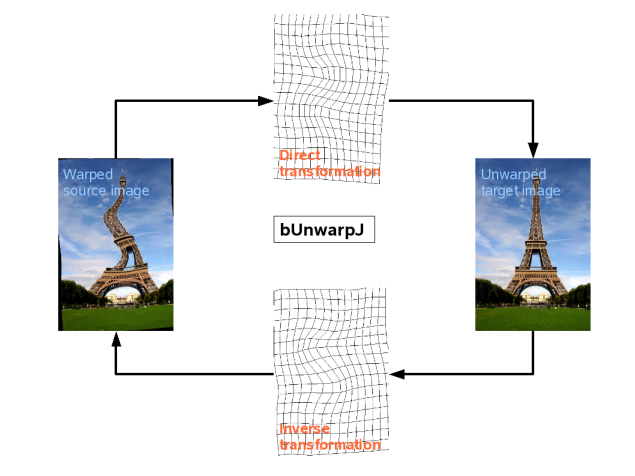
\includegraphics[width=\textwidth]{figures/Chapter_1/BUnwarpJ_scheme.png}
	\caption{Illustration of the bUnwarpJ algorithm principle}
	\label{fig:scheme_bunwrapJ}
\end{figure}

This image registration algorithm is based on the minimization of an energy functional that includes the dissimilarity between the source and target images -in both directions- $E_{img}$, an optional landmark constraint $E_{\mu}$, a regularization term $(E_{div} + E_{rot})$, and an energy term $E_{cons}$ that accounts for the geometrical consistency between the elastic deformation in both directions. Namely, the energy function is given by:
\begin{equation*}
		E = w_iE_{img} + w_{\mu}E_{\mu} + (w_dE_{div} + w_rE_{rot}) + w_cE_{cons} 
\end{equation*}
                  

Where the weights of every term are set by the user in the main window of the plugin. The optimization process is a Levenberg-Marquardt minimization enhanced by a Broyden-Fletcher-Goldfarb-Shanno (BFGS) estimate of the local Hessian of the goal function, and both, images and deformations are represented by cubic B-splines \cite{bunwrapJ,unwrapJ}. 

\paragraph{}
Once the deformation matrix and its inverse extracted from the calibration step, each inverse transformation matrix $A(P)$ is applied to the $image(P)$ recorded during the spring experiment. The resulting image corresponds to an image recorded using a non-deformed tank window.\\
All this process was automatized, using a script written in ImageJ macro language.
\subsubsection{Contour extraction algorithm}
\paragraph{}
Once the distortion corrected, we needed to extract from each image three physical quantities:
\begin{enumerate}
	\item Elongation of the spring.
	\item Shape and volume of the capsule.
	\item Gravity center of the capsule.
\end{enumerate}
\paragraph{}
An algorithm was written in python, based on an image treatment library called "`Opencv"', to automatically extract the three quantities for each image, following these steps, enriched by illustrations at each step applied to a raw image, in the buckling state, which represents the most complex  situation (fig.\ref{fig:raw_image}):
\begin{figure}[H] %
	\centering%
  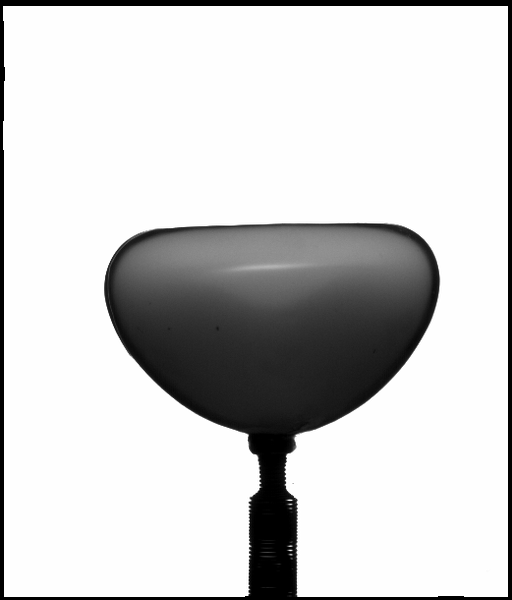
\includegraphics[width=0.48\textwidth]{figures/Chapter_1/raw_image.png}
	\caption{Raw image used for the illustrations}
	\label{fig:raw_image}
\end{figure}
\paragraph{}
First, the image is cropped to the boundaries of the displacement of the capsule during the experiment, to reduce memory and space disk consumption.
\paragraph{}
Second, the resulting image is filtered (fig.\ref{fig:filtering_image_treatment}), using two types of filters: a Gaussian filter where each point in the input array is convolved with a Gaussian kernel and then summing them all to produce the output array. Gaussian blurring is highly effective in removing Gaussian noise from the image. The second, is a median filter, which runs through each element of the image and replace each pixel with the median of its neighboring pixels. it is highly effective against salt-and-pepper noise in the images.
The filtering kernel size were kept to a low level, to avoid dilatation of the pixels and an alteration of the capsule's contour.

\begin{figure}[H]%
	\centering%
	 \begin{subfigure}[h]{0.48\textwidth}%
        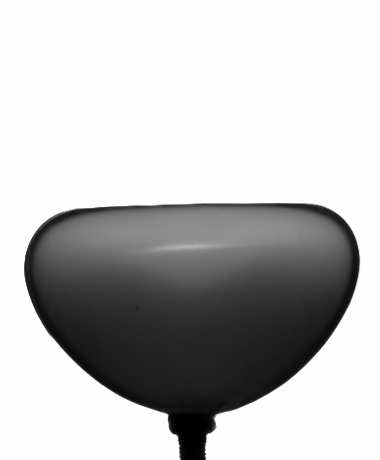
\includegraphics[width=\linewidth]{figures/Chapter_1/median_b.png}%
        \caption{Median blurring}%
				\label{fig:median_f}%
    \end{subfigure}%
    \begin{subfigure}[h]{0.48\textwidth}%
        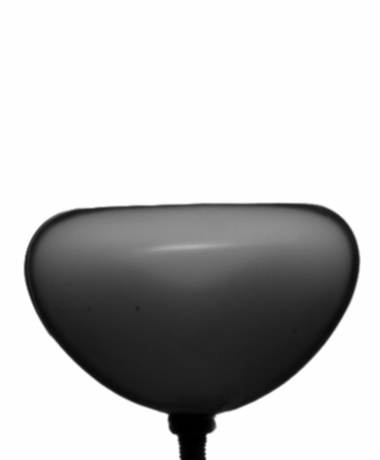
\includegraphics[width=\linewidth]{figures/Chapter_1/gaussian_b.png}%
        \caption{Gaussian blurring}%
        \label{fig:gaussian_f}%
    \end{subfigure}%
		
		\begin{subfigure}[h]{0.48\textwidth}%
        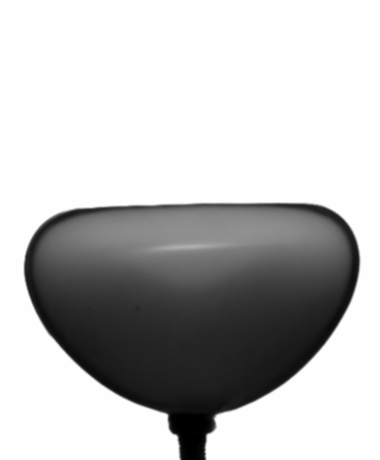
\includegraphics[width=\linewidth]{figures/Chapter_1/resulting_f.png}%
        \caption{resulting filtered image}%
				\label{fig:resulting_f}%
    \end{subfigure}%
		\caption{Filtering technique and results}%
		\label{fig:filtering_image_treatment}%
\end{figure}
\paragraph{}
Third, canny edge detector algorithm\cite{canny} is used to find the edges on the image (fig.\ref{fig:canny}). Briefly, this algorithm relies on finding the intensity gradients of the image, thinning the edge, by using the "`non-maximum suppression"' technique, and then applying a double threshold to get rid of the noise.
\begin{figure}[H] %
	\centering%
  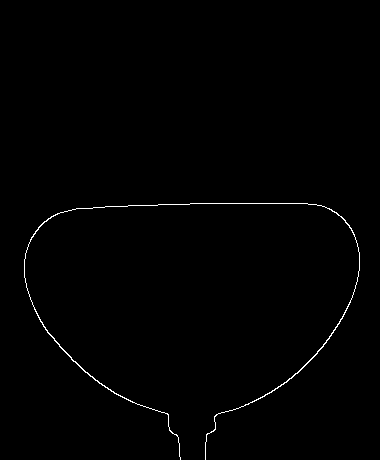
\includegraphics[width=0.48\textwidth]{figures/Chapter_1/canny.png}
	\caption{Canny edge detection}
	\label{fig:canny}
\end{figure}
\paragraph{}
From the canny image (fig.\ref{canny}), the white pixels are extracted, to get the general contour. Then, the capsule shape is extracted, by first, determining the maximum horizontal distance "`maxD"' between two white points, this distance is close to the maximum width of the ball. Knowing the y-position of "`maxD"', and exploiting the monotonous decrease of the horizontal distance, at higher y (the origin being the top left pixel), we can remove the spring shape by setting a minimum horizontal distance, as shown in figure \ref{fig:ball_shape}.

\begin{figure}[H] %
	\centering%
  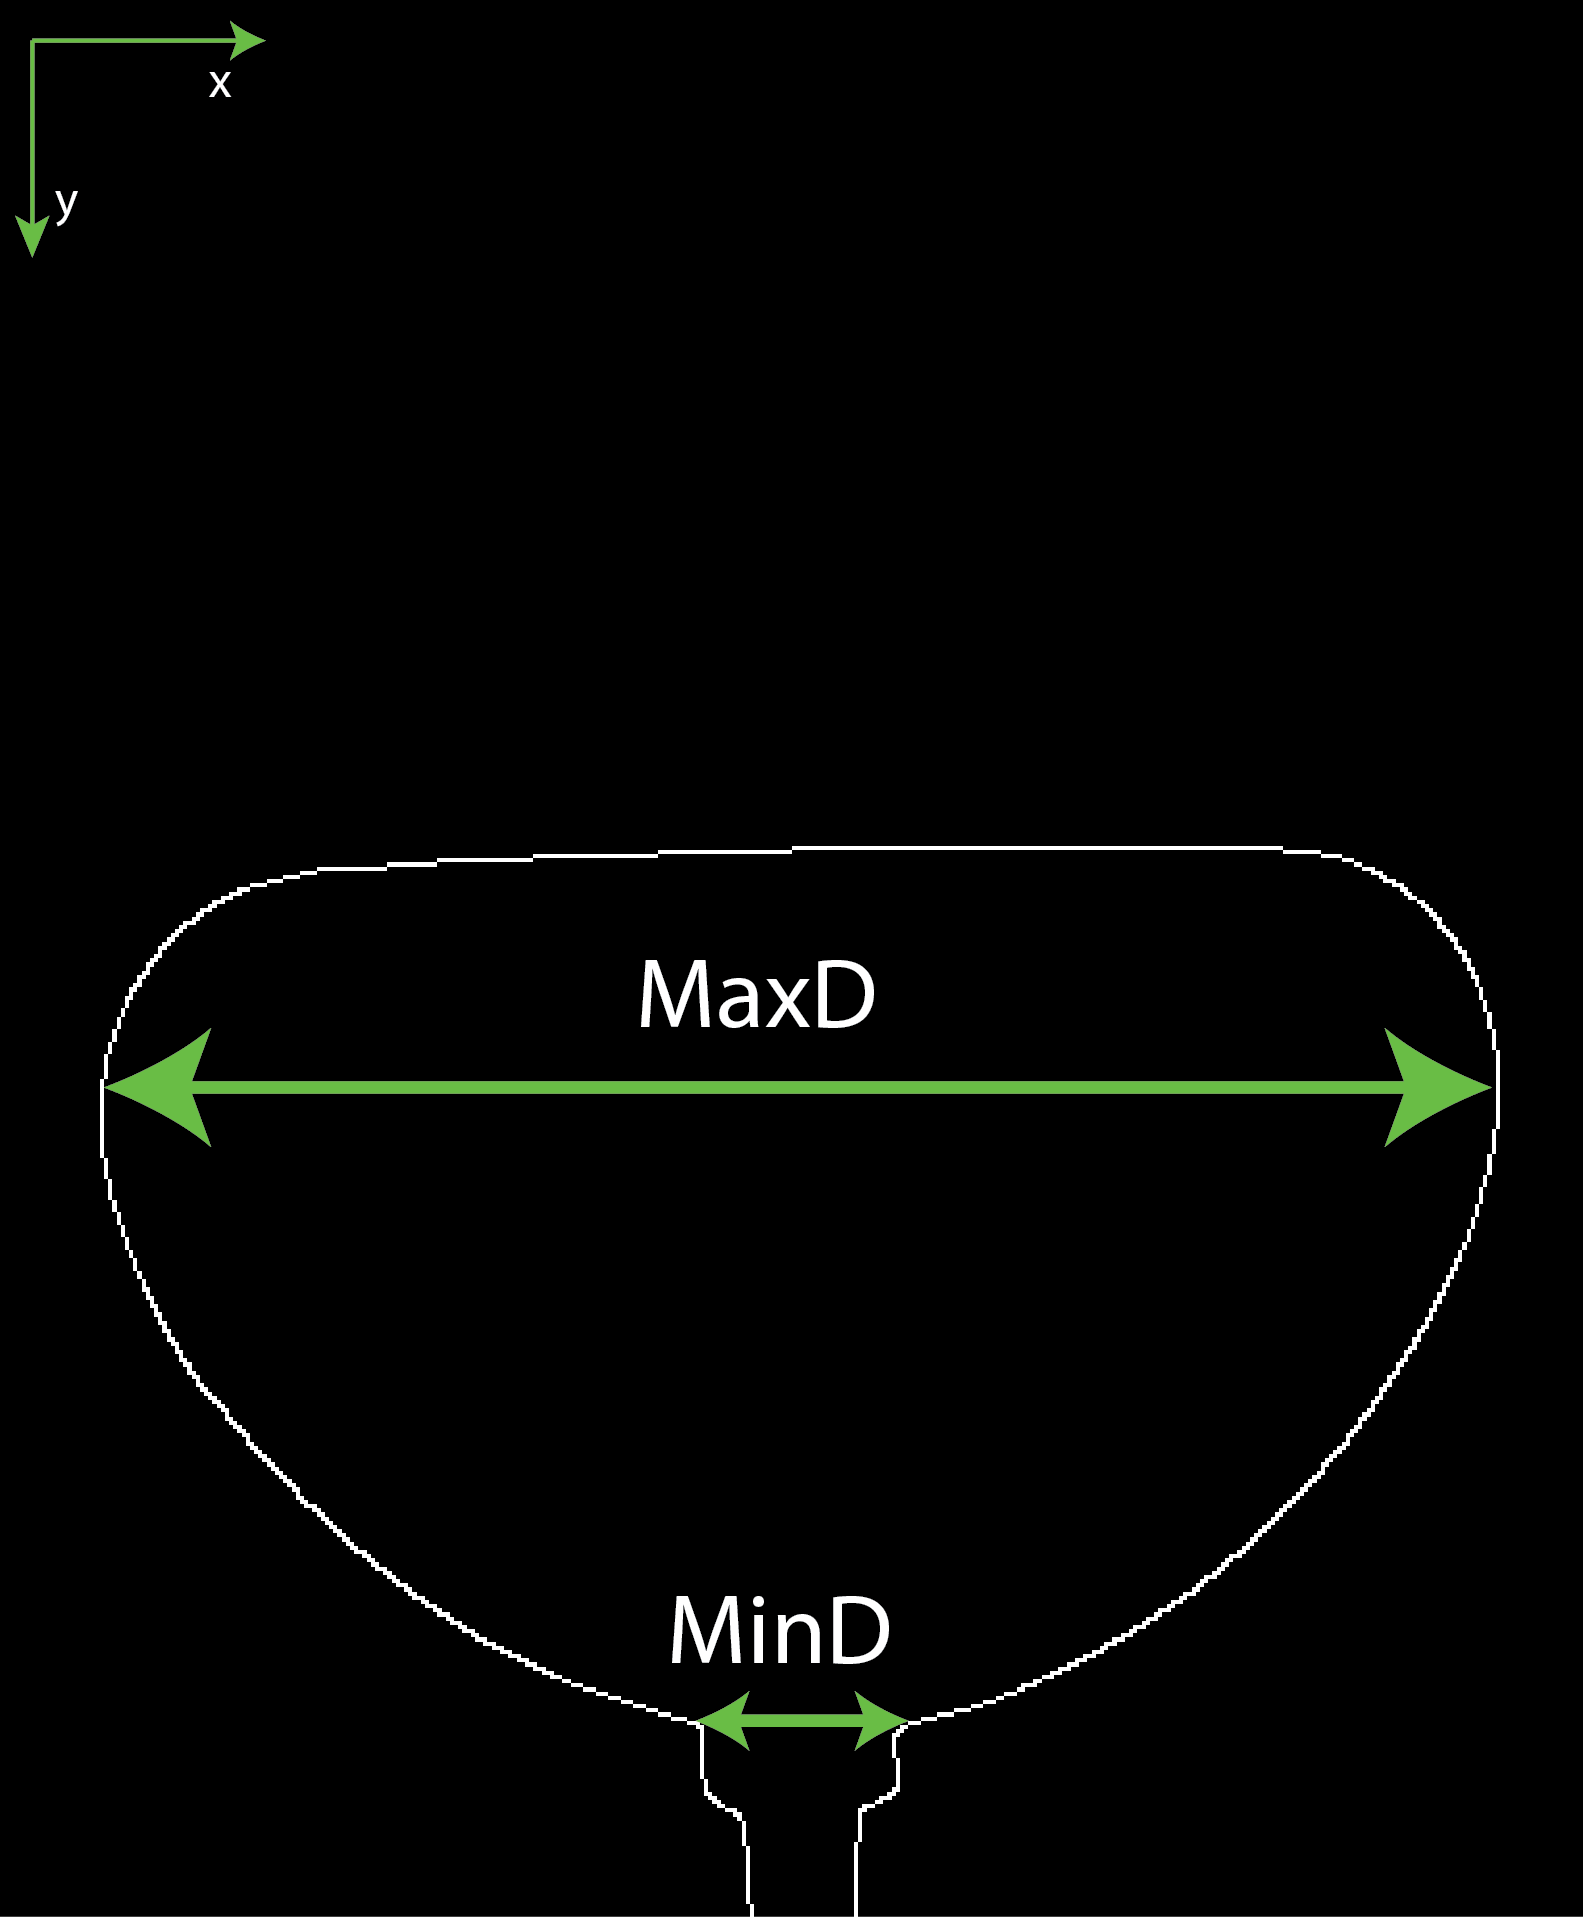
\includegraphics[width=\textwidth]{figures/Chapter_1/ball_shape.png}
	\caption{Ball shape}
	\label{fig:ball_shape}
\end{figure}
\paragraph{}
Once the ball shape defined, its outer contour is fitted with a parametric curve, defined in the polar coordinates system, proceeding as follow:
\begin{enumerate}
	\item Define an initial center $M_{c0} (x_{c0},y_{c0})$ to the polar coordinate system, as being the mean value of the experimental points constituting the ball shape.
	\begin{align*}
			x_{c0} &= \frac{\sum\limits_{i=1}^N x_i}{N} \\
			y_{c0} &= \frac{\sum\limits_{i=1}^N y_i}{N} \\
	\end{align*}
	Where $x_i$ and $y_i$ are the coordinates of the experimental points, and $N$ being the number of points.
	\item Define an iterative process which minimizes the difference between a fitting parametric curve and the experimental points,where at each iteration, the 		following operations are performed: 
	
		\begin{enumerate}[label=\alph*)]
			\item Transform every experimental point from the cartesian coordinates system  $M(x,y)$ to the polar coordinates system $M'(R,\theta)$  as follow:
				\begin{align*}
				R_{exp}(\theta)_i &=\sqrt{(x_i- x_c)^2+(y_i-y_c)^2}  \\
				\theta_{exp}_i &= \arctan(\frac{y_i-y_c}{x_i- x_c}) \\
				\end{align*}
				Where $x_c$ and $y_c$ are fitting parameters corresponding to the center of the polar coordinates, initialised by $M_{c0} (x_{c0},y_{c0})$.
			\item Evaluate the fitting parametric curve:
				\begin{align*}
					\tilde{R}_(\theta)_i &=\sum\limits_{k=0}^M a_k \sin(\theta_{exp}_i-\theta_0)^k  \\
				\end{align*}
				for the fitting parameters $\theta_0$\footnote{$\theta_0$ represents the angle formed bet ween the symetry axis of the experimental points and the y-axis.} 			 and $a_k$ coefficients, with $k={0,...,M}$, $M$ being the degree of the polynomial.
			\item Measure the distance $R_exp(\theta)_i-\tilde{R}_(\theta)_i$ and iterate.
		\end{enumerate}
	The minimization is done using "`Levenberg-Marquardt"' method, commonly known as "`least_squares"' minimization method.
	\item The iterative process stops when reaching a residual smaller than a given threshold.	
\end{enumerate}
\paragraph{}
\begin{figure}[H] %
	\centering%
  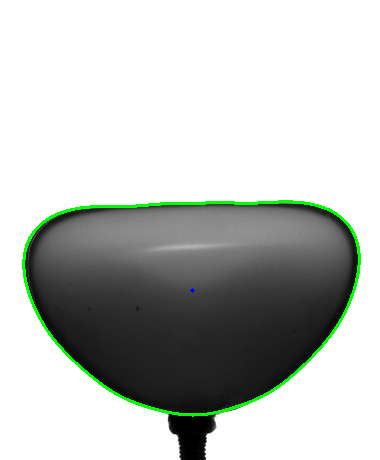
\includegraphics[width=0.48\textwidth]{figures/Chapter_1/outer_contour.png}
	\caption{Fitted outer contour in green, and center of the parametric curve in blue}
	\label{fig:outer_contour}
\end{figure}
Once the outer contour fitted (fig.\ref{fig:outer_contour}), the experimental points defining the concavity are extracted from the image automatically. A region of interest (ROI) where the concavity occurs is defined around the maximum diameter region (fig\ref{fig:concavity_extraction}. Canny edge detector, is then applied to the ROI.
\begin{figure}[H] %
	\centering%
  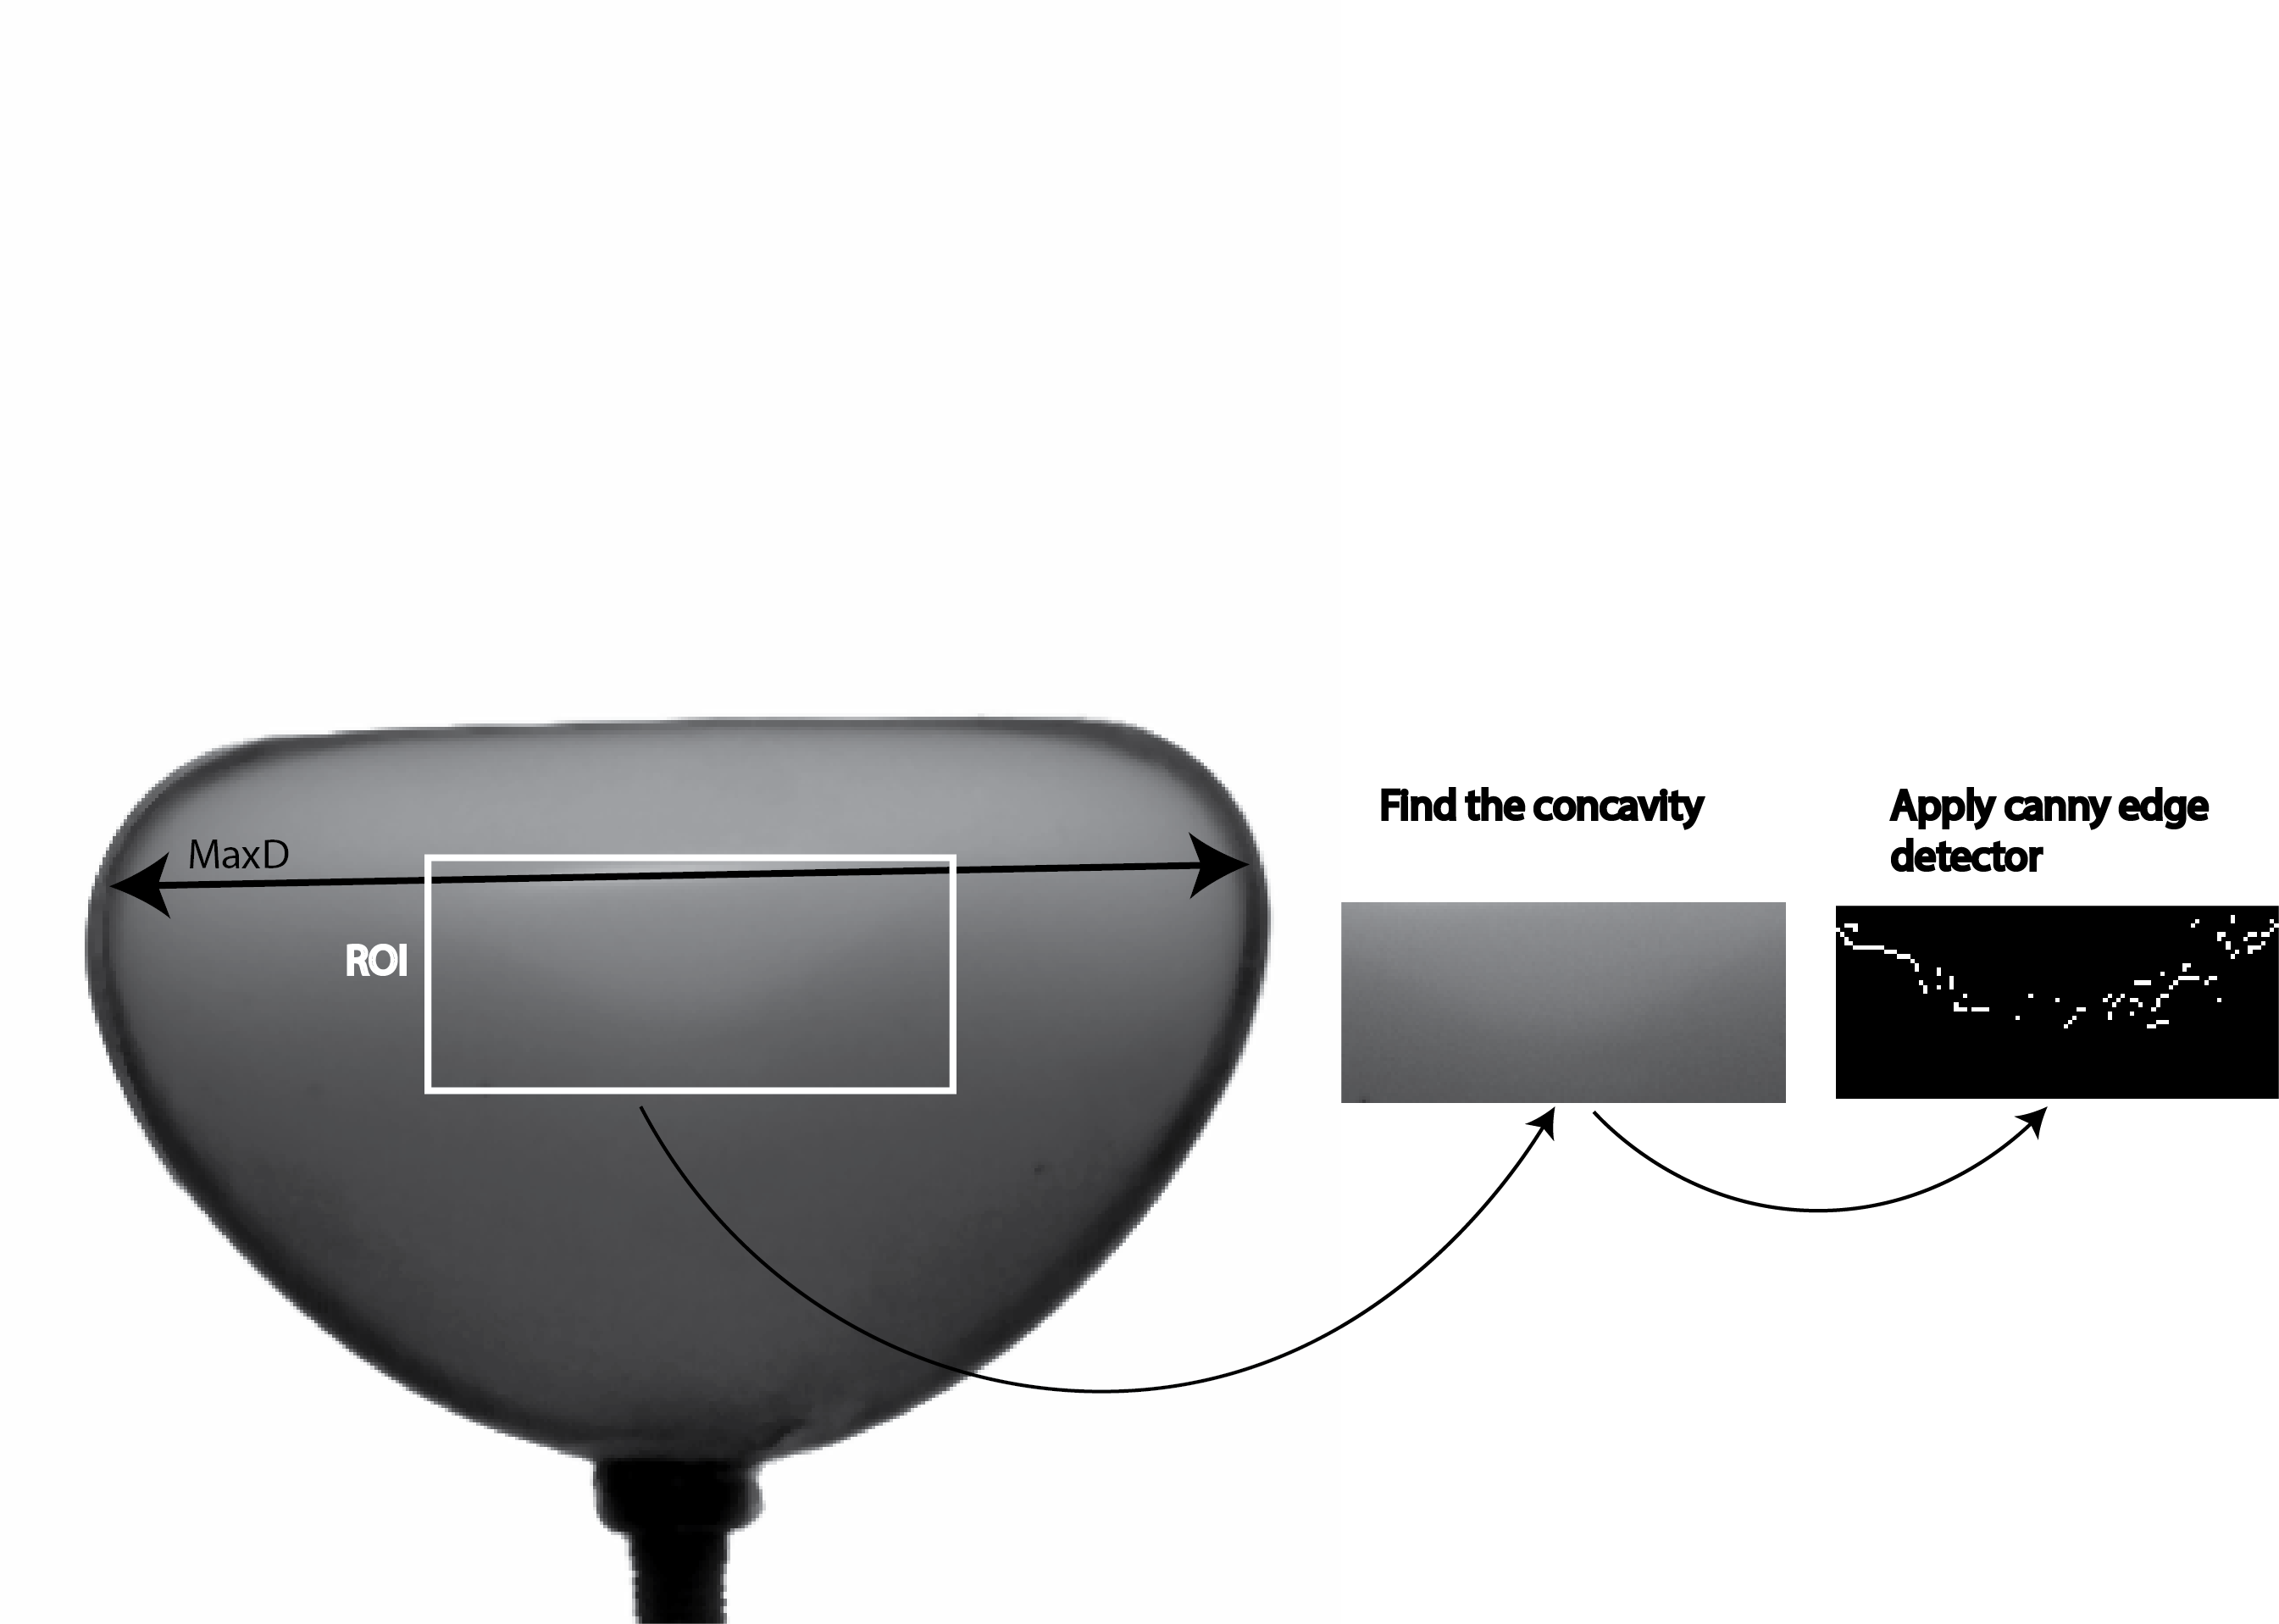
\includegraphics[width=0.48\textwidth]{figures/Chapter_1/concavity_extraction.png}
	\caption{Extraction of the concavity experimental points}
	\label{fig:concavity_extraction}
\end{figure}
\paragraph{}
To create a complete fit between the outer contour and a fit of the concavity, we need first, to cut the outer contour where it ceases to belong to the shape generatrix, which generates the physical surface of the concave capsule. This limit is set by the point of the parametric outer curve where the tangent is horizontal.
Practically, it means, find the point $M(R_{h},\theta_h)$, such as the the following condition is respected:
\begin{equation}
	\tan(\theta+\alpha) &=0\\
	\label{eq:tangent_horizontal}
\end{equation}
Where $\alpha$^is the angle defined between the tangent line $T$ with the vector $\vec{OM}$ (see fig.\ref{fig:Illustration_tangent}), defined as such:
\begin{equation}
	\tan(\alpha) &=|{\frac {\tilde{R}(\theta )}{\tilde{R}'(\theta )}}|\\
	\label{eq:tangent}
\end{equation}
\begin{figure}[H] %
	\centering%
  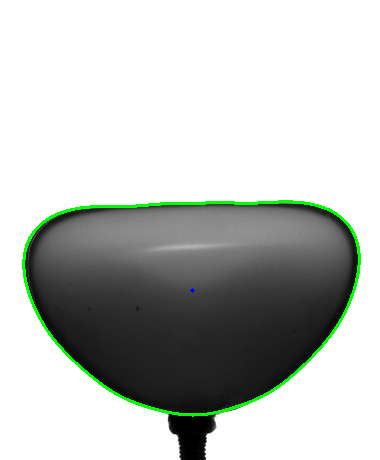
\includegraphics[width=0.48\textwidth]{figures/Chapter_1/outer_contour.png}
	\caption{Fitted outer contour in green, and center of the parametric curve in blue}
	\label{fig:outer_contour}
\end{figure}
Integrating \eqref{eq:tangent} in \eqref{eq:tangent_horizontal}, gives a condition an equation on theta:
\begin{align*}
	\tan(\theta+\alpha) &=0\\
	\\Rightarrow\\
	\frac{\tan(\theta)+\tan(\alpha)}{1-\tan(\theta)\tan(\alpha)} &= 0\\
	\\Rightarrow\\
	\tan(\theta)+\tan(\alpha) &= 0\\
	\\Rightarrow\\
	\tan(\theta)+|{\frac {\tilde{R}(\theta )}{\tilde{R}'(\theta )}}|&=0
	\\Rightarrow\\
	\tan(\theta)+|{\frac {\sum\limits_{k=0}^M a_k \sin(\theta)^k  )}{\cos(\theta) \sum\limits_{k=1}^M k a_k \sin(\theta)^(k-1) )}}|&=0
\end{align*}
The point $M(R_{h},\theta_h)$ is determined by minimizing this final expression.\\
The outer contour belonging to the shape generatrix is defined as:
\begin{align*}
	\tilde{R}(\theta) &= \sum\limits_{k=0}^M a_k \sin(\theta)^k, \intertext{with } \theta \in[-\pi-\theta_h,\theta_h]
	\theta
\end{align*}
Now, we need to fit the concavity experimental points with a functional which guaranties the continuity and differentiability at the $M(R_{h},\theta_h)$ point.\\
To do so, we define a fitting functional as follows:
\begin{align*}
g(y) &= a x^6+b x^4+ c x^2+ d\\
\intertext{with the following continuity conditions on $d$ and $c$}
d &= -c x_{c}^2 - b x_{c}^4 -ax_{c}^6+ y_c\\
\intertext{and}
c &= -2 b x_{c}^2-3 a x_{c}^4
\end{align*}
Where $a,b,c,d$ are the fit parameters, and $x_c,y_c$ are the coordinates of the point $M(R_{h},\theta_h)$ in the cartesian coordiantes system, based around the center of the polar coordinate system, previously defined.\\
\paragraph{}
The combination of the two fits, determines an analytical description of the generatrix (fig.\ref{fig:fit_complet}), allowing the analytical calculus of the volume and the center of gravity of the capsule\footnote{The calculus of these two quantities being complex, is not developed here and can be found in the annexe.}. 
%as follow:\\
%For the volume:
%\begin{align*}
	%V_{shape} &= V_{outer_contour}+V{concavity}\\
	%\intertext{Where:}
	%V_{outer_contour} & = \frac{2\pi}{3} \sum\limits_{i,j,k=0}^M a_i a_j a_k(\frac{1.-(\cos(\phi_h))^{(i+j+k)}}{(1.+i+j+k)})
	%\intertext{With:}
	%\phi_h &=\frac{\pi}{2}-\theta_h\\
	%\intertext{and: }
	%V{concavity} &= 2\pi((\sum\limits_{i=0}^3 \frac{1}{2(i+1)}x_c^{2(i+1)})-\frac{\tan(\phi_h)*x_c^3}{3})
%\end{align*}
%and for the gravity center:
%\begin{align*}
	%V_{shape} &= V_{outer_contour}+V{concavity}\\
	%\intertext{Where:}
	%V_{outer_contour} & = \frac{2\pi}{3} \sum\limits_{i,j,k=0}^M a_i a_j a_k(\frac{1.-(\cos(\phi_h))^{(i+j+k)}}{(1.+i+j+k)})
	%\intertext{With:}
	%\phi_h &=\frac{\pi}{2}-\theta_h\\
	%\intertext{and: }
	%V{concavity} &= 2\pi((\sum\limits_{i=0}^3 \frac{1}{2(i+1)}x_c^{2(i+1)})-\frac{\tan(\phi_h)*x_c^3}{3})
%\end{align*}

\begin{figure}[H] %
	\centering%
  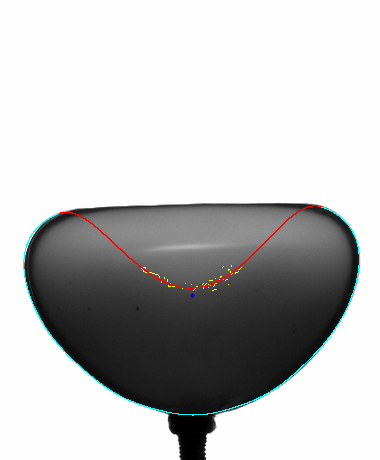
\includegraphics[width=0.48\textwidth]{figures/Chapter_1/outer_contour_complete.png}
	\caption{Fitted outer contour in blue, fitted concavity in red, and experimental concavity points in yellow}
	\label{fig:fit_complet}
\end{figure}
\paragraph{Note}
In the case of a convex shape, only the outer contour fit is considered.



